%\documentclass[11pt,draftcls,onecolumn]{IEEEtran}
\documentclass[10pt,twocolumn,twoside]{IEEEtran}

\usepackage{amstext}
\usepackage{amsmath}
\usepackage{amssymb}
\usepackage{graphicx}
\usepackage{epstopdf}
\usepackage{algorithm}
\usepackage{algorithmic}
\usepackage{booktabs}
\usepackage[tight]{subfigure}
\usepackage{comment, color}

% correct bad hyphenation here
\hyphenation{op-tical net-works semi-conduc-tor}

\input IEEE_RMT_MSD_header.tex

% Figure size
\newcommand{\figwidth}{2.5in}

\begin{document}
%
% paper title
% can use linebreaks \\ within to get better formatting as desired
\title{The Performance of a Matched Subspace Detector that Uses Subspaces Estimated from Finite, Noisy, Training Data}


\author{Nicholas~Asendorf
        and~Raj~Rao~Nadakuditi\\
%EDICS: SSP-DETC, SSP-PERF% <-this % stops a space

\thanks{Copyright (c) 2012 IEEE. Personal use of this material is permitted. However, permission to use this material for any other purposes must be obtained from the IEEE by sending a request to pubs-permissions@ieee.org.}

\thanks{N. Asendorf is with the Department
of Electrical Engineering and Computer Science, 1301 Beal Avenue, Room 4313, University of Michigan, Ann Arbor,
MI, 48109 USA (e-mail: asendorf@umich.edu).}% <-this % stops a space
\thanks{R.R. Nadakuditi is with the Department
of Electrical Engineering and Computer Science, 1301 Beal Avenue, Room 4118, University of Michigan, Ann Arbor,
MI, 48109 USA (e-mail: rajnrao@umich.edu).}% <-this % stops a space
\thanks{Manuscript received ??}}

% The paper headers
\markboth{IEEE Journal,~Vol.~?, No.~?, ?~?}%
{Asendorf and Nadakuditi: The Performance of a Matched Subspace Detector that Uses Subspaces Estimated from Finite, Noisy, Training Data}
% The only time the second header will appear is for the odd numbered pages
% after the title page when using the twoside option.
%
% *** Note that you probably will NOT want to include the author's ***
% *** name in the headers of peer review papers.                   ***
% You can use \ifCLASSOPTIONpeerreview for conditional compilation here if
% you desire.

% make the title area
\maketitle


\begin{abstract}
We analyze the performance of a matched subspace detector (MSD) where the test signal vector is assumed to reside in an unknown, low-rank $k$ subspace that must be estimated from finite, noisy, signal-bearing training data. Under both a stochastic and deterministic model for the test vector, subspace estimation errors due to limited training data degrade the performance of the standard plug-in detector, relative to that of an oracle detector. To avoid some of this performance loss, we utilize and extend recent results from random matrix theory (RMT) that precisely quantify the quality of the subspace estimate as a function of the eigen-SNR, dimensionality of the system, and the number of training samples. We exploit this knowledge of the subspace estimation accuracy to derive from first-principles a new RMT detector and to characterize the associated ROC performance curves of the RMT and plug-in detectors. Using more than the a critical number of \textit{informative} components, which depends on the training sample size and eigen-SNR parameters of training data, will result in a performance loss that our analysis quantifies in the large system limit.  We validate our asymptotic predictions with simulations on moderately sized systems.

\end{abstract}

% Note that keywords are not normally used for peerreview papers.
\begin{IEEEkeywords}
Matched subspace detector, deterministic, stochastic, random matrix theory, ROC analysis
\end{IEEEkeywords}


\IEEEpeerreviewmaketitle

\section{Introduction}\label{sec:intro}
% Old version
%\IEEEPARstart{M}{any} signal processing  \cite{scharf1991statistical} and machine learning \cite{friedman2001elements} applications involve the task of detecting a signal of interest buried in high dimensional noise. A matched subspace detector (MSD) is commonly used to solve this problem when the target signal is assumed to lie in a low-rank subspace.  The low-rank signal buried in noise model is ubiquitous in signal processing. See for example, \cite{besson2006cfar,bandiera2007glrt, bandiera2007adaptive}, which determine if a snapshot is noise-only or if it contains target echoes, \cite{maris2003resampling, soong1995principal}, which examine source localization in electroencephalography (EEG) and magnetoencephalography (MEG) data, and \cite{besson2005matched}, which examines low-rank signal recovery in radar, sonar, and communications applications. The performance of such detectors when the signal subspace is known a priori has been extensively studied (see, for example, \cite{besson2006cfar,scharf1994matched,jin2005cfar,mcwhorter2003matched, vincent2008matched} to list a few). This paper considers the performance of a MSD in the less studied setting where the signal subspace is unknown and must be estimated from finite, noisy, signal-bearing training data.

\IEEEPARstart{M}{any} signal processing  \cite{scharf1991statistical} and machine learning \cite{friedman2001elements} applications involve the task of detecting a signal of interest buried in high dimensional noise. A matched subspace detector (MSD) is commonly used to solve this problem when the target signal is assumed to lie in a low-rank subspace.  The low-rank signal buried in noise model is ubiquitous in signal processing. In array processing, \cite{besson2005matched} and \cite{besson2006cfar} use multiple array snapshots to detect a low-rank signal in the presence of both interference and noise when the noise power is known and unknown, respectively. Similarly in adaptive radar detection, \cite{bandiera2007adaptive} and \cite{bandiera2007glrt} adaptively detect distributed low-rank targets given multiple snapshots of primary (signal plus noise) and secondary (noise only) data under partially homogeneous and homogeneous noise assumptions, respectively. Low rank signal models are also used in electroencephalography (EEG) and magnetoencephalography (MEG) source localization as in \cite{maris2003resampling} and \cite{soong1995principal}, respectively. In \cite{besson2005matched,besson2006cfar,bandiera2007adaptive,bandiera2007glrt}, the signal subspace is known. The performance of a MSD when the signal subspace is known was studied in \cite{scharf1994matched} and \cite{vincent2008matched} under deterministic signal assumptions and in \cite{mcwhorter2003matched} and \cite{jin2005cfar} under stochastic signal assumptions. This paper considers the performance of a MSD in the less studied setting where the signal subspace is unknown and must be estimated from finite, noisy, signal-bearing training data.

The setting we have in mind arises from machine learning related applications where the low-rank signal model is reasonable but the signal subspace is not parameterizable. This is in contrast to the array processing applications that motivated the original MSD work \cite{scharf1994matched} where the signal subspace is explicitly parameterizable whenever the array geometry is known. The inferential problem is made tractable by the availability of a training dataset consisting of signal-bearing observations that have been collected in a variety of representative experimental (and thus noisy) conditions. In such a scenario,  the truncated eigen-decomposition of the sample covariance matrix of this training data yields an estimate of the unknown low-rank signal subspace, which may then be used for signal versus noise discrimination.

An illustrating example of this is the classical problem of handwriting recognition \cite[Chapter 10]{elden2007matrix} where a MSD can be used to determine if an area of an image contains a digit $0-9$ or is pure noise. Here, a database \cite{hwritingurl}, containing a large number of handwritten samples of each of the digits written by many different writers, is used to form a low-rank subspace estimate of each digit. The samples are noisy because of digitization effects and the inherent variation between writers. A nearest-subspace classifier based on retaining only the first few ($10-12$, in this example) principal components (or leading eigenvectors of the digit's training data sample covariance matrix) associated with each digit yields greater than 93\% classification performance \cite[Table 10.1, pp. 121]{elden2007matrix}, indicating that the low-rank signal buried in noise model is appropriate. The motivating setting described also arises in the context of image or wavefront recognition applications (e.g. license plate character recognition) where the target and the camera are separated by a dynamic random medium and in hyperspectral imaging based anomaly detection  \cite{thai2002invariant,healey1999models,kwon2006kernel} relative to a statistically stationary scene (e.g. toxic gas detection). Here too, a practitioner might have access to training samples collected over a variety of experimental conditions and might employ the MSD in a similar manner.

In these applications, the standard plug-in detector, which substitutes an estimate of the signal subspace into the expression for the oracle MSD that was derived assuming the subspace is perfectly known, realizes a performance loss because additive noise and finite training data decrease the accuracy of the estimated subspace. This motivates questions such as: What is the expected plug-in detector performance? Is it possible to avoid some of this performance loss? How does the estimation of the signal subspace dimension influence detector  performance? Is the ``play-it-safe''  overestimation of subspace dimension, to compensate for the potential underestimation of schemes discussed in \cite{nadakuditi2008sample} , a good idea? 

Our performance analysis, which relies on insights from random matrix theory (RMT), highlights the importance of using no more than $\keff$ \textit{informative} signal subspace components, where $\keff$ is a number that depends on the system dimensionality, number of training samples, and eigen-SNR (signal-to-noise-ratio). We derive a new RMT detector that only utilizes the $k_\text{eff}$ \textit{informative} signal subspace components, thereby avoiding some of the possible performance loss suffered by the plug-in detector. Given the number and quality (i.e. SNR) of the training samples, our analysis also allows a practitoner to predict the expected receiver operating characteristic (ROC) performance of a general class of detectors. An outcome of this analyis is that we can accurately predict how many training samples are needed to get to within $\epsilon$ of the oracle MSD's performance (see Figures \ref{fig:epsilon_graph}, \ref{fig:stoch_theory_epsilon}, and \ref{fig:determ_theory_epsilon}). This performance characterization can provide the practitioner with experimental guidance and might be a starting point for the formulation of achievable system performance specifications.

This paper differs from previous works in several aspects. The focus and main contribution is analytically quantifying the performance of a general class of MSD's as a function of the system dimensionality, number of training samples, and eigen-SNR. Theorem \ref{th:other angles} and Corollary \ref{corr:matrix} extend recent results from RMT \cite{paul2007asymptotics,benaych2011eigenvalues, benaych2011singular} to precisely quantify the accuracy of the subspace estimate. This quantification yields approximations that appear to hold for moderate system dimensions even though the theory is asymptotic, in the limit of large dimensionality and relatively large training sample size. We provide a first-principles derivation of a new RMT detector that incorporates this knowledge of the accuracy of the estimated subspace, thereby illuminating the asymptotic form of a detector that mitigates some of the potential performance loss suffered by the plug-in detector. These RMT insights also allow us to characterize the ROC performance of a MSD under both a deterministic and stochastic model for the test vector. This work builds on \cite{asendorf2011msd} by providing the proofs of Theorem \ref{th:other angles} and Corollary \ref{corr:matrix}, analyzing the performance of the general class of detectors given in (\ref{eq:detector_form}), considering the deterministic test vector setting, and unifying the performance analysis of the stochastic and deterministic MSD's.

The paper is organized as follows. We describe the generative models for the training data and test vector and also estimate unknown parameters in Section \ref{sec:data_models}. In Section \ref{sec:std_detecs}, we derive standard oracle and plug-in detectors for each testing setting and highlight how finite training data causes subspace estimation errors and subsequent performance loss. We formally pose the questions addressed herein in Section \ref{sec:prob_state}. Section \ref{sec:rmt} contains pertinent results from RMT and our definition in (\ref{eq:keff}) of $\keff$. In Section \ref{sec:rmt_detecs} we derive RMT detectors for the stochastic and deterministic test vector models. Aided by RMT and a saddlepoint approximation of the CDF of a weighted sum of chi-square random variables, we predict ROC performance curves for a general detector in Section \ref{sec:roc_theory}. We validate our asymptotic ROC predictions and demonstrate the importance of using the $k_\text{eff}$ informative subspace components in Section \ref{sec:results}. We provide concluding remarks in Section \ref{sec:conclusion}.







\section{Data Models and Parameter Estimation}\label{sec:data_models}
\textcolor{blue}{Given an observation, we wish to discriminate between the $H_0$ hypothesis that the observation is purely noise and the $H_1$ hypothesis that the observation contains a target signal. We assume that the signal of interest lies in a low dimensional subspace as in \cite{besson2006cfar,bandiera2007glrt,bandiera2007adaptive,maris2003resampling,soong1995principal,besson2005matched,thai2002invariant, healey1999models,kwon2006kernel}. However, this low-rank subspace and the SNR governing the subspace components are unknown. To design a detector to distinguish between the $H_0$ and $H_1$ hypotheses, we have access to a training dataset, recorded under similar noisy conditions, whose observations are known to contain the signal of interest (see, for example, \cite{healey1999models,kwon2006kernel}). We use this training data to form estimates of the unknown low-rank subspace and each component's SNR. This section will mathematically describe the training data models, how we estimate any unknown parameters, and a stochastic and deterministic model for the testing data. Both testing models share the same training data model.}

\subsection{Training Data Model}\label{sec:training_data}

\textcolor{blue}{We model our unknown subspace with the complex matrix $U=[u_1,\dots,u_k]$ such that $\dim u_i = n$ and $\langle u_i, u_j\rangle = u_i^Hu_j=\delta_{ij}$ for $i,j=1,\dots,k$. Here $\delta_{ij}$ is the delta function such that $\delta_{ij} = 0$ for $i\neq j$ and $\delta_{ij}=1$ for $i=j$.} We are given $m$ signal-bearing training vectors $y_i\in \complex^{n\times 1}$, $i=1,\dots,m$, modeled\footnote{For expositional simplicity, we have assumed that all our matrices and vectors are complex-valued; our results also hold for real-valued matrices and vectors.} as $y_i=Ux_i+z_i$ where $z_i\overset{\text{i.i.d.}}{\sim}\mathcal{CN}(0,I_n)$ and $x_i\overset{\text{i.i.d.}}{\sim}\mathcal{CN}(0,\Sigma)$ where $\Sigma=\diag(\sigma_1^2,\dots,\sigma_k^2)$ with $\sigma_1>\sigma_2>\dots>\sigma_k>0$ unknown. \textcolor{blue}{Similar gaussian priors appear in \cite{bandiera2007glrt, bandiera2007adaptive,thai2002invariant, healey1999models}}. $\Sigma$ models the SNR of each subspace component and $z_i$ models the additive noise. For each observation, $x_i$ and $z_i$ are independent. The dimension, $k$, of our subspace is unknown and we assume throughout that $k\ll n$ so that we have a low-rank signal embedded in a high-dimensional observation vector.

\subsection{Parameter Estimation}\label{sec:param_estim}

\textcolor{blue}{The parameters $k$, $U$, and $\Sigma$ are all unknown in our training model. For the rest of the paper, we assume that we are given a dimension estimate, $\widehat{k}$; this may have been estimated from the training data or provided by a domain expert. Typically, $\widehat{k}$ is an overestimation of a dimension estimate provided by percent variance, scree plots \cite{zhu2006automatic}, or robust techniques \cite{nadakuditi2010fundamental,johnstone2001distribution,el2007tracy}. This overestimation, or ``play-it-safe'' strategy, strives to include all signal subspace components at the expense of possibly including non-signal subspace compoents.}

\textcolor{blue}{Given $\widehat{k}$ and the signal bearing training data $Y = \begin{bmatrix} y_1 & \dots & y_m \end{bmatrix}$, we form the sample covariance matrix $S=\frac{1}{m}YY^{H}$. The covariance matrix of $y_i$ is $U\Sigma U^H +I_n$ and it follows that the (classical) ML estimates (in the many-sample, small matrix setting) for $U$ and $\Sigma$ are given by \cite{muirhead1982aspects}
\begin{equation}\label{eq:param_estims_stoch}
\begin{aligned}
&\widehat{U}=[\widehat{u}_1 \dots \widehat{u}_{\widehat{k}}]\\
&\textcolor{blue}{\widehat{\sigma}_i^2 = \max(0,\widehat{\lambda}_i -1)} \text{ for } i=1,\dots,\widehat{k}\\
\end{aligned}
\end{equation}
where $\widehat{\lambda}_1,\dots,\widehat{\lambda}_{\widehat{k}}$ are the $\widehat{k}$  largest eigenvalues of the sample covariance matrix, $S$, and $\widehat{u}_1,\dots,\widehat{u}_{\widehat{k}}$ are the corresponding eigenvectors. Define the signal covariance matrix estimate as $\widehat{\Sigma}=\diag(\widehat{\sigma}_1^2,\dots,\widehat{\sigma}_{\widehat{k}}^2)$. We are now able to use the parameter estimates $\widehat{U}$ and $\widehat{\Sigma}$ in detectors where necessary.}

\subsection{Testing Data Model}
\textcolor{blue}{We will consider both a stochastic and deterministc model for a test vector. In both settings, parameter estimates are formed as described in (\ref{eq:param_estims_stoch}) from training data modeled in Section \ref{sec:training_data}.}

In the stochastic setting, the test vector $y\in\complex^{n\times 1}$ is modeled as
\small\begin{equation}\label{eq:stoch_setup}
\text{Stochastic Model: }y=\left\{
\begin{aligned}
&z
&& y\in H_0:\text{ Noise only}\\
&Ux+z
&& y\in H_1:\text{ Signal-plus noise}\\
\end{aligned}\right. ,
\end{equation}\normalsize
where $U$, $z$, and $x$ are modeled as described in Section \ref{sec:training_data}. This assumes that the signal, $Ux$, may lie anywhere in the subspace and whose position in the subspace is governed by the signal covariance matrix $\Sigma$.

In the deterministic setting, the test vector $y\in\complex^{n\times 1}$ is modeled as
\small\begin{equation}\label{eq:determ_setup}
\text{Deterministic Model: }y=\left\{
\begin{aligned}
&z
&& y\in H_0:\text{ Noise only}\\
&U\Sigma^{1/2} x+z
&& y\in H_1:\text{ Signal-plus noise}\\
\end{aligned}\right. ,
\end{equation}\normalsize
where $U$, $\Sigma$, and $z$ are modeled as described in Section \ref{sec:training_data}. Here, in contrast to the stochastic setting, $x$ is a non-random deterministic vector. Thus the signal, $U\Sigma^{1/2}x$, lies at a fixed point in the unknown subspace. \textcolor{blue}{Note that $\Sigma$ still controls the SNR of each subspace component} and that placing a mean zero, identity covariance Gaussian prior on $x$ in (\ref{eq:determ_setup}) yields the stochastic model described in (\ref{eq:stoch_setup}).


\section{Standard Detector Derivations}\label{sec:std_detecs}
In this paper, we focus on the  Neyman-Pearson setting (see \cite{van1968detection}) where, given a test observation from (\ref{eq:stoch_setup}) or (\ref{eq:determ_setup}), a MSD is a likelihood ratio test (LRT) taking the form
\begin{equation}\label{eq:lrt}
\Lambda(y):=\dfrac{f(y|H_1)}{f(y|H_0)} \detgtrless \eta
\end{equation}
where $\Lambda(y)$ is the test statistic, $\eta$ is the threshold set to achieve a given false alarm rate, and $f$ is the appropriate conditional density of the test observation. In the following section, for both testing data models we derive the standard oracle detector (assuming all parameters are known) and plug-in detector (formed by substituting the parameter estimates of (\ref{eq:param_estims_stoch}) in the oracle detector). The oracle detectors, while unrealizable, give an upper bound for the performance of a MSD. We will see that when only finite training data is available (as is the case in real applications), the plug-in detector will realize a performance loss relative to this bound.

\subsection{Stochastic Testing Model}\label{sec:plugin_stoch}
The LRT in (\ref{eq:lrt}) depends on the conditional distribution of the test vector, $y$. By properties of Gaussian random variables, when using the stochastic test model in (\ref{eq:stoch_setup}), these distributions are $y|H_0\sim\mathcal{N}\left(0,I_n\right)$ and $y|H_1\sim\mathcal{N}\left(0, U\Sigma U^H +I_n\right)$. The resulting LRT statistic is
\begin{equation}\label{eq:stoch_lrt}
\Lambda(y)=\frac{\mathcal{N}(0,U\Sigma U^H + I_n)}{\mathcal{N}(0,I_n)}.
\end{equation}
We derive an oracle detector by assuming that $k$, $\Sigma$, and $U$ are all known in (\ref{eq:stoch_lrt}). After simplification of this expression (see Section 4.14 of \cite{scharf1991statistical}), the oracle statistic becomes
\begin{equation}\label{eq:oracle_stat_stoch_y}
\Lambda_{\text{oracle}}(y) = y^HU\left(\Sigma^{-1}+I_k\right)^{-1}U^Hy.
\end{equation}
Note that the oracle statistic depends on the sufficient statistic $w:=U^Hy$. Using this notation, the oracle statistic is
\begin{equation}\label{eq:oracle_stat_stoch_w}
\boxed{\Lambda_{\text{oracle}}(w) = w^H\left(\Sigma^{-1}+I_k\right)^{-1}w = \sum_{i=1}^k\left(\frac{\sigma_i^2}{\sigma_i^2+1}\right)w_i^2}
\end{equation}
and the oracle detector is $\Lambda_{\text{oracle}}(w) \detgtrless \gamma_{\text{oracle}}$
where the threshold $\gamma_{\text{oracle}}$ is chosen in the usual manner, \ie, so that it satisfies $P(\Lambda_{\text{oracle}}(w)>\gamma_{\text{oracle}}|H_0)=\alpha$ with $\alpha$ a desired false alarm rate.

However, as the parameters $U$ and $\Sigma$ are unknown, the oracle statistic in
(\ref{eq:oracle_stat_stoch_w}) cannot be computed. Given a dimension estimate
$\widehat{k}$, we substitute the ML estimates of $U$ and $\Sigma$ given in
(\ref{eq:param_estims_stoch}) for the unknown parameters in (\ref{eq:oracle_stat_stoch_y})
as similarly done in \cite{mcwhorter2003matched} and \cite{jin2005cfar}. This results in the plug-in detector's LRT statistic: $
\Lambda_{\text{plugin}}(y)= y^H\widehat{U}\left(\widehat{\Sigma}^{-1}+I_{\widehat{k}}\right)^{-1}\widehat{U}^Hy$. Simplifying this expression using the statistic $\widehat{w} = \widehat{U}^Hy$, yields the plug-in statistic
\begin{equation}\label{eq:plugin_stat_stoch}
\boxed{\Lambda_{\text{plugin}}(\widehat{w}) = \widehat{w}^H\diag\left(\frac{\widehat{\sigma}^2_i}{\widehat{\sigma}^2_i+1}\right)\widehat{w}=\sum_{i=1}^{\widehat{k}}\left(\frac{\widehat{\sigma}_i^2}{\widehat{\sigma}_i^2+1}\right)\widehat{w}_i^2}
\end{equation}
and the plug-in detector takes the form $\Lambda_{\text{plugin}}(w) \detgtrless \gamma_{\text{plugin}}$
%\begin{equation}\label{eq:plugin_class_stoch}
%\Lambda_{\text{plugin}}(w) \detgtrless \gamma_{\text{plugin}}
%\end{equation}
where the threshold $\gamma_{\text{plugin}}$ is chosen in the usual manner.

The plug-in detector assumes that the estimated signal subspace, $\widehat{U}$, is equal to the true signal subspace, $U$, and that the estimated signal covariance, $\widehat{\Sigma}$, is equal to the true signal covariance, $\Sigma$. In other words,  the plug-in detector derivation assumes that $\widehat{U}^HU=I_{\widehat{k}}$, $\widehat{\sigma}_i^2=\sigma_i^2$ for $i=1,\dots,\widehat{k}$, and the provided subspace dimension estimate, $\widehat{k}$, is equal to the true underlying dimension of our signal subspace, $k$. Perhaps unsurprisingly, (as discussed in Section \ref{sec:rmt}) incorrectly choosing $\widehat{k}$ degrades the performance of the plug-in detector.

\subsection{Deterministic Testing Model}\label{sec:plugin_determ}
We now consider the alternative deterministic test vector model (\ref{eq:determ_setup}), which results in the following conditional distributions of the test vector $y|H_0\sim\mathcal{N}(0,I_n)$ and $y|H_1\sim\mathcal{N}(U\Sigma^{1/2} x, I_n)$. We begin by deriving an oracle detector, which assumes that $U$, $\Sigma$, $x$, and $k$ are all known. The LRT statistic for such a scenario is $\Lambda(y) = \frac{\mathcal{N}(U\Sigma^{1/2} x, I_n)}{\mathcal{N}(0,I_n)}$. Simplifying this expression leads to the oracle statistic
\begin{equation}\label{eq:determ_stat_oracle_y}
\Lambda_{\text{oracle}}(y) = x^H\Sigma^{1/2}U^Hy.
\end{equation}
As in the stochastic setting, $w=U^Hy$ is a sufficient statistic and the oracle statistic simplifies to
\begin{equation}\label{eq:determ_stat_oracle_w}
\boxed{\Lambda_{\text{oracle}}(w) = x^H\Sigma^{1/2}w = \sum_{i=1}^kx_i\sigma_iw_i.}
\end{equation}

However, as the parameters $U$, $\Sigma$, and $x$  are unknown, the oracle statistic in (\ref{eq:determ_stat_oracle_w}) cannot be computed. Since we must estimate $x$ from the test vector, we employ the generalized likelihood ratio test (GLRT) where $\Lambda(y) = \frac{\max_x f(y|H_1)}{f(y|H_0)}$, resulting in the GLRT statistic
\begin{equation}\label{eq:glrt_determ}
\Lambda(y)=\frac{\max_x\mathcal{N}(U\Sigma^{1/2} x,I_n)}{\mathcal{N}(0,I_n)}.
\end{equation}
Employing maximum likelihood estimation on $x$ in (\ref{eq:glrt_determ}) yields the estimate $\widehat{x}=\Sigma^{-1/2}U^Hy$.  Proceeding as in the stochastic setting, we substitute $\widehat{x}$ for the unknown $x$ in (\ref{eq:determ_stat_oracle_y}) and then substitute the ML estimates of $U$ and $\Sigma$ given in (\ref{eq:param_estims_stoch}) for the unknown $U$ and $\Sigma$ (see Section 4.11 of \cite{scharf1991statistical} for a similar treatment). This results in the plug-in statistic $\Lambda_{\text{plugin}}(y) = y^H\widehat{U}\widehat{U}^Hy$. Again, $\widehat{w}=\widehat{U}^Hy$ is a statistic that can be used to write the plug-in statistic as
\begin{equation}\label{eq:plugin_stat_determ}
\boxed{\Lambda_{\text{plugin}}(\widehat{w}) = \widehat{w}^H\widehat{w}=\sum_{i=1}^{\widehat{k}}\widehat{w}_i^2},
\end{equation}
resulting in the detector $\Lambda_{\text{plugin}}(\widehat{w}) \detgtrless \gamma_{\text{plugin}}$, 
%\begin{equation}\label{eq:plugin_class_determ}
%\Lambda_{\text{plugin}}(\widehat{w}) \detgtrless \gamma_{\text{plugin}},
%\end{equation}
where the threshold $\gamma_{\text{plugin}}$ is chosen in the usual manner. The deterministic plug-in detector is an `energy detector', which sums the energy of the test observation lying in the subspace $\widehat{U}$.

\subsection{Effect of the Number of Training Samples}\label{sec:training_effect}
In both the stochastic and deterministic testing settings, $\widehat{w}=\widehat{U}^Hy$ is a statistic used in the plug-in statistics (\ref{eq:plugin_stat_stoch}) and (\ref{eq:plugin_stat_determ}). This statistic relies on the estimated subspace $\widehat{U}$ formed from the top $\widehat{k}$ eigenvectors of the sample covariance matrix, $S$, of the training data. The stochastic detector also relies on the subspace-SNR estimate $\widehat{\Sigma}$ formed from the top $\widehat{k}$ eigenvalues of $S$. For a fixed $\Sigma$, the accuracy of these estimates depends on the number of training data samples, $m$; we will mathematically show this in Section \ref{sec:rmt}. If we had access to an infinite amount of training data, the parameter estimates would be exact ($\widehat{U}\to U$ and $\widehat{\Sigma}\to\Sigma$). However, when we have access to only a finite amount of training data, $\widehat{U}$ and $\widehat{\Sigma}$ are inaccurate and will degrade the performance of the plug-in detectors with respect to the oracle detector, which provides an upper bound on detector performance.

\begin{figure}[t]
\centering
\subfigure[Stochastic Setting]{
\includegraphics[width=\figwidth]{figures/asend1a.pdf}
\label{fig:stoch_oracle}
}
\subfigure[Deterministic Setting]{
\includegraphics[width=\figwidth]{figures/asend1b.pdf}
\label{fig:determ_oracle}
}
\vspace{-0.1in}
\caption{Empirical ROC curves for the plug-in and oracle detectors. Empirical ROC curves were simulated with $n=200$, $\widehat{k}=k=2$, and $\Sigma =\diag\left(10,0.1\right)$. The empirical ROC curves were computed using $10000$ test samples and averaged over 100 trials using algorithms 2 and 4 of \cite{fawcett2006introduction}. (a) Shows results for the stochastic MSD. (b) Shows results for the deterministic MSD when $x=[0.75,0.75]^T$. For both settings, as $m$ decreases, the performance of the plug-in detector degrades.}
\label{fig:plugin_v_oracle}
\vspace{-0.3in}
\end{figure}

To illustrate this performance loss, we consider a moderately sized system where $n=200$ and $\Sigma=\diag(10,0.1)$. We consider five detectors: the oracle detector and four plug-in detectors each using parameter estimates formed from varying amounts of training data. Figures \ref{fig:stoch_oracle} and \ref{fig:determ_oracle} plot the empirical ROC curves for the stochastic and deterministic testing settings, respectively. The amount of training data drastically affects the performance of the plug-in detector. As $m$ decreases, the plug-in detectors realize a significance performance loss. However, as $m\to\infty$, the plug-in detectors realize improved performance, closer to that of the oracle detectors.

For the stochastic detector, as $m\to\infty$, the plug-in detector achieves the same performance as the oracle detector. Examination of the statistics (\ref{eq:oracle_stat_stoch_w}) and (\ref{eq:plugin_stat_stoch}) shows that these statistics will be identical when $\widehat{U}\to U$ and $\widehat{\Sigma}\to\Sigma$, which is the case when infinite training data is available. However, this is not the case for the deterministic plug-in detector. Even with an infinite amount of training data, the plug-in detector will not achieve the oracle detector's performance. The deterministic plug-in detector must estimate $x$ given a noisy test observation $y$, which is independent from the training data. Even with infinite training data causing $\widehat{U}\to U$ and $\widehat{\Sigma}\to\Sigma$, $\widehat{x}$ does not converge to $x$. Therefore, the deterministic plug-in detector cannot achieve the performance bound of the oracle detector, which assumes that $x$ is known.

For a fixed probability of false alarm ($P_F$), we can explore this performance loss by comparing the achieved probability of detection ($P_D$) of the plug-in detector to that of the oracle detector. Let
\begin{equation}\label{eq:epsilon}
\epsilon = 1 - \frac{P_D^{\text{plugin}}}{P_D^{\text{oracle}}}
\end{equation}
be the performance loss of the plug-in detector. Figure \ref{fig:epsilon_graph} empirically plots the number of training samples needed to achieve a desired performance loss $\epsilon$ for the stochastic plug-in detector. There is an exponential relationship between $\epsilon$ and $m$ indicating that we need infinite training samples to achieve zero performance loss ($\epsilon=0$). However, in any practical application we will never have an infinite amount of training data and so the plug-in detector will realize some non-zero performance loss. The rest of the paper will mathematically predict how finite training data affects detector performance and will derive new detectors to avoid some of this performance loss.

\begin{figure}[t]
\centering
\includegraphics[width=\figwidth]{figures/asend2.pdf}
\vspace{-0.1in}
\caption{Empirically determined number of training samples, $m$,  needed for the stochastic plug-in detector to achieve a desired performance loss, $\epsilon$, as defined in (\ref{eq:epsilon}). The required false alarm rate is $P_F=0.1$. Empirical ROC curves were generated for $n=200$, $\Sigma=\diag(10,0.1)$, $\widehat{k}=k=2$ using 10000 testing samples and averaged over 100 trials using algorithms 2 and 4 of \cite{fawcett2006introduction}.}
\label{fig:epsilon_graph}
\vspace{-0.3in}
\end{figure}


\section{Problem Statements}\label{sec:prob_state}
\input{prob_state.tex}

\section{Pertinent Results from Random Matrix Theory}\label{sec:rmt}
We are given signal-bearing training data $\{y_1,\dots,y_m\}$ where $y_i\in H_1$ for $i=1,\dots,m$ from which we obtain estimates $\widehat{U}$ and $\widehat{\Sigma}$ of the unknown $U$ and $\Sigma$. Consider the $n \times m$ data matrix $Y = \begin{bmatrix} y_1 & \ldots & y_m \end{bmatrix}$. The eigenvalue decomposition of the sample covariance matrix, $S=\frac{1}{m}YY^H$ yields the maximum likelihood estimates of $U$ and $\Sigma$.


\subsection{Eigenvector Aspects}

Specifically, assuming $k$ is known, we set $\widehat{U}$ to equal the $n \times k$ matrix whose columns are the $k$ eigenvectors associated with the $k$ largest eigenvalues of $S$. We now quantify the accuracy of the estimated eigenvectors.\\

\begin{prop}\label{th:angles}
Assume that the columns of the training data matrix $Y$ were generated as described in Section \ref{sec:training_data}. Let $\widehat{u}_{i}$ denote the eigenvector associated with the $i$-th largest eigenvalue of $S$. Then for $i = 1, \ldots, k$ and $n, m \longrightarrow \infty$ with $n/m \to c$, we have that
\begin{equation}
|\langle u_i,\widehat{u}_i\rangle|^2 \convas
\begin{cases}
\dfrac{\sigma_i^4-c}{\sigma_{i}^4+\sigma_{i}^2c} & \text{ if } \sigma_{i}^2>\sqrt{c}\\
0 & \textrm{otherwise}\\
\end{cases}.
\end{equation}
\end{prop}
\begin{proof}
This result appears in \cite{paul2007asymptotics,benaych2011eigenvalues}.
\end{proof}


The key insight from Proposition \ref{th:angles} is that only the eigenvectors corresponding to the signal eigenvalues lying above the phase transition $\sqrt{c}$ are \textit{informative}. When a signal eigenvalue drops below this critical threshold, the corresponding eigenvector estimate is essentially noise-like  (i.e. $|\langle u_i,\widehat{u}_i\rangle|^2=o_{p}(1)$) and thus \textit{uninformative}.

The term $|\langle u_i,\widehat{u}_i\rangle|^2$ quantifies mismatch between the estimated and underlying eigenvectors and will play an important role in deriving a new detector and in characterizing detector performance; a similar term also comes up in the analysis of the resolving power of arrays due to model mismatch such as in \cite{cox1973resolving}.


Following \cite{nadakuditi2008sample}, we define the effective number of identifiable subspace components $k_\text{eff}$ as:
\begin{equation}\label{eq:keff}
\boxed{k_\text{eff} = \text{Number of } \sigma_i^2 > \sqrt{c}}.
\end{equation}
We can estimate $k_\text{eff}$ using, for example,  `Algorithm 2' of  \cite{nadakuditi2010fundamental}. We now state an additional theorem that will prove useful in our derivations.\\

\begin{Th}\label{th:other angles}
Assume the same hypothesis as in Proposition \ref{th:angles}. Then for fixed $k$ and  $i,j = 1, \ldots, k $ and $n, m \longrightarrow \infty$ with $n/m \to c$, we have that for $i \neq j$,
\begin{equation}
\langle u_j,\widehat{u}_i\rangle \convas 0.
\end{equation}
\end{Th}
\begin{proof}
In the Appendix we prove the statement for $i, j = 1, \ldots, \keff$. The proof for the setting where $i, j > \keff$ is considerably more involved and we omit it here for space considerations.
\end{proof}\vskip0.25cm

Matrices of the form $\widehat{U}^HU D U^H\widehat{U}$ will appear throughout our derivations in Sections \ref{sec:msd_stoch}, \ref{sec:msd_determ}, and \ref{sec:roc_theory}. We apply Proposition \ref{th:angles} and Theorem \ref{th:other angles} to state a result that permits approximation, in the large matrix limit, of  $\widehat{U}^HU D U^H\widehat{U}$ by a suitable diagonal matrix.  \\
%Intuitively, we expect the performance of detectors which utilize subspace components for which $|\langle u_i,\widehat{u}_i\rangle|^2=o_{p}(1)$ to be suboptimal.

\begin{Corr}\label{corr:matrix}
Suppose $\widehat{k}\leq k$ and let $D$ be a $k \times k$ (non-random) diagonal matrix such that $D=\diag(d_1,\ldots,d_{k})$, independent of $\widehat{U}$. Then as $n,m \longrightarrow \infty$ with $n/m \to c$, we have that
\begin{equation*}
\widehat{U}^HU D U^H\widehat{U}\convas \diag(d_1 |\langle u_1,\widehat{u}_1\rangle|^2,\dots, d_{\widehat{k}} |\langle u_{\widehat{k}},\widehat{u}_{\widehat{k}}\rangle|^2)
\end{equation*}
where for $i=1,\dots,\widehat{k}$ the quantity $|\langle u_i,\widehat{u}_i\rangle|^2$ is given in Proposition \ref{th:angles}.
\end{Corr}

\subsection{Eigenvalue Aspects}

Random matrix theory also provides insights about the accuracy of the eigenvalues of $S$, as described next.
\begin{prop}\label{th:high_eigvals}
As $n,m \longrightarrow \infty$ with $n/m \to c$, when $\sigma_i^2 > \sqrt{c}$, we have that:
\begin{equation*}
\widehat{\sigma}_i^2\convas \sigma_i^2 + c + \frac{c}{\sigma_i^2}.
\end{equation*}
\end{prop}
\begin{proof}
See Theorem 2 in \cite{paul2007asymptotics} for the real setting when $c<1$ and \cite{benaych2011singular} for the complete result.
\end{proof}
This estimate is clearly biased and we now characterize the fluctuations on the signal variance estimate.
\begin{prop}\label{th:eigenvalues}
As $n,m \longrightarrow \infty$ with $n/m \to c$, we have that for $i = 1, \ldots, \keff$
\begin{equation*}
\sqrt{n}\left(\widehat{\sigma}_i^2-\left(\sigma_i^2+c+\frac{c}{\sigma_i^2}\right)\right)\Rightarrow\mathcal{N}\left(0,\frac{2\left(\sigma_i^2+1\right)^2}{\beta }\left(1-\frac{c}{\sigma_i^4}\right)\right),
\end{equation*}
where $\beta = 1$ when the data is real-valued and $\beta = 2$ when the data is complex-valued.
\end{prop}
\begin{proof}
See Theorem 3 in \cite{paul2007asymptotics} for the real setting when $c<1$ and \cite{benaych2011singular} for the complete result.
\end{proof}
We form an improved estimate of the unknown signal variance, $\sigma_{i}^{2}$, by employing maximum-likelihood (ML) estimation on the distribution in Proposition \ref{th:eigenvalues}. Specifically, for only the $k_\text{eff}$ signal eigenvalues, we form the estimate:
\begin{equation}\label{eq:cov}
\widehat{\sigma}^2_{i_\text{rmt}} = \argmax_{\sigma_i^2} \log\left(f_{\widehat{\sigma}_i^2}(\sigma_i^2)\right)
\end{equation}
where
\begin{equation*}
f_{\widehat{\sigma}_i^2}(\sigma_i^2):=\mathcal{N}\left(\left(\sigma_i^2+c+\frac{c}{\sigma_i^2}\right),\frac{2\left(\sigma_i^2+1\right)^2}{n\beta }\left(1-\frac{c}{\sigma_i^4}\right)\right).
\end{equation*}
We may then estimate $|\langle u_i,\widehat{u}_i\rangle|^2$ by substituting the improved signal variance estimates, $\widehat{\sigma}^2_{i_\text{rmt}}$, for the unknown $\sigma_i^2$ in Proposition \ref{th:angles}. We refer to this estimate as $|\langle u_i,\widehat{u}_i\rangle|^2_{\text{rmt}}$. For the $\max(0,\widehat{k}-k_\text{eff})$ uninformative subspace components, we set $|\langle u_i,\widehat{u}_i\rangle|^2_{\text{rmt}}=0$. We estimate the signal variances under the phase transition by invoking the following result.\\

\begin{prop}\label{th:low_eigvals}
As $n,m \longrightarrow \infty$ with $n/m \to c$, when $\sigma_i^2 \leq \sqrt{c}$, we have that:
\begin{equation*}
\widehat{\sigma}_i^2\convas c + 2\sqrt{c}.
\end{equation*}
\end{prop}
\begin{proof}
See Theorem 1 in \cite{paul2007asymptotics} for the real setting when $c<1$ and \cite{benaych2011singular} for the complete result.
\end{proof}

We use (\ref{eq:cov}) and Propositions \ref{th:angles}, \ref{th:high_eigvals}, and \ref{th:low_eigvals} to derive theoretical ROC curves in Section \ref{sec:roc_theory}.


\section{Derivation of New RMT Matched Subspace Detectors}\label{sec:rmt_detecs}
\input{rmt_detecs.tex}

%\section{Family of Stochastic Matched Subspace Detectors}\label{sec:msd_stoch}
%%%%%We now derive a family of detectors for the stochastic observation vector model in (\ref{eq:stoch_setup}). Recall that we form a test vector $w=\widehat{U}^Hy$; the elements of $w$ are the `co-ordinates' of $y$ in the subspace spanned by the columns of $\widehat{U}$. In the Neyman-Pearson setting, the oracle detector is a LRT which relies on the conditional distributions of our test vector $w$ under each hypothesis. By properties of Gaussian random variables these distributions are simply
\begin{equation}\label{eq:stoch_distr}
\begin{aligned}
&w|H_0\sim\mathcal{N}\left(0,I_{\widehat{k}}\right)\\
&w|H_1\sim\mathcal{N}\left(0, \widehat{U}^HU\Sigma U^H\widehat{U} +I_{\widehat{k}}\right).\\
\end{aligned}
\end{equation}
We obtain a family of detectors by placing various assumptions on the covariance of $w|H_1$, as described next.
%Given a dimension estimate $\widehat{k}$, $\widehat{U}$ is a $n\times\widehat{k}$ matrix formed by stacking the top $\widehat{k}$ eigenvectors of the sample covariance matrix of the training data alongside each other.

\subsection{Oracle Detector}\label{sec:oracle_stoch}
The oracle detector assumes that $k$, $\Sigma$, and $\widehat{U}^{H}U$ are all known in (\ref{eq:stoch_distr}). The LRT statistic is
\begin{equation*}
\Lambda(w)=\frac{\mathcal{N}(0,\widehat{U}^HU\Sigma U^H\widehat{U} + I_k)}{\mathcal{N}(0,I_{k})}.
\end{equation*}
After simplification of this expression using the natural logarithm operator as a monotonic operation, the oracle statistic becomes
\begin{equation}\label{eq:oracle_stat_stoch}
\boxed{\Lambda_{\text{oracle}}(w) = w^H\left[I_k-\left(\widehat{U}^HU\Sigma U^H\widehat{U}+I_k\right)^{-1}\right]w}
\end{equation}
and the oracle detector is
\begin{equation}\label{eq:oracle_class_stoch}
\Lambda_{\text{oracle}}(w) \detgtrless \gamma_{\text{oracle}}
\end{equation}
where the threshold $\gamma_{\text{oracle}}$ is chosen in the usual manner, \ie, so that satisfies $P(\Lambda_{\text{oracle}}(w)>\gamma_{\text{oracle}}|H_0)=\alpha$ with $\alpha$ a desired false alarm rate. We note that the oracle statistic assumes that the matrix $\widehat{U}^HU\Sigma U^H\widehat{U}$ is known. \textcolor{blue}{Corollary \ref{corr:matrix} states that in the large system limit, this matrix converges almost surely to a diagonal matrix showing that asymptotically the oracle detector is of the form given by (\ref{eq:detector_form})}.  We exploit this in Section \ref{sec:optimal_stoch} to address the problem posed in Section \ref{sec:ps_prob2}.

\subsection{Plug-in Detector}\label{sec:plugin_stoch}
When the parameters $\Sigma$ and $U$ (and the implicit variable $k$) in (\ref{eq:stoch_distr}) are unknown, the expression in (\ref{eq:oracle_stat_stoch}) cannot be computed. Given a dimension estimate $\widehat{k}$ we form parameters estimates of $U$ and $\Sigma$ as in (\ref{eq:param_estims_stoch}). We then substitute these ML estimates for the unknown parameters in (\ref{eq:oracle_stat_stoch}) as in \cite{jin2005cfar} and \cite{mcwhorter2003matched}. \textcolor{blue}{This results in the following plug-in detector LRT statistic:}
\begin{equation*}
\textcolor{blue}{\Lambda_{\text{plugin}}(w)= w^H\left(I_{\widehat{k}}-\left[\widehat{U}^H\widehat{U}\widehat{\Sigma}\widehat{U}^H\widehat{U} + I_{\widehat{k}}\right]^{-1}\right)w.}
\end{equation*}
This simplifies to
\begin{equation}\label{eq:plugin_stat_stoch}
\boxed{\Lambda_{\text{plugin}}(w) = w^H\diag\left(\frac{\widehat{\sigma}^2_i}{\widehat{\sigma}^2_i+1}\right)w=\sum_{i=1}^{\widehat{k}}\left(\frac{\widehat{\sigma}_i^2}{\widehat{\sigma}_i^2+1}\right)w_i^2}
\end{equation}
and our detector takes the form
\begin{equation}\label{eq:plugin_class_stoch}
{\Lambda_{\text{plugin}}(w) \detgtrless \gamma_{\text{plugin}}}
\end{equation}
where the threshold $\gamma_{\text{plugin}}$ is chosen in the usual manner. The stochastic plug-in detector clearly takes the form of (\ref{eq:detector_form}).

The plug-in detector assumes that the estimated signal subspace, $\widehat{U}$, is equal to the true signal subspace, $U$, and that the estimated signal covariance, $\widehat{\Sigma}$, is equal to the true signal covariance, $\Sigma$. In other words,  the plug-in detector derivation assumes that $|\langle u_i,\widehat{u}_i\rangle|^2=1$ and $\widehat{\sigma}_i^2=\sigma_i^2$ and that the provided subspace dimension estimate, $\widehat{k}$, is equal to the true underlying dimension of our signal subspace, $k$. Perhaps unsurprisingly, (as discussed in Section \ref{sec:rmt}) choosing $\widehat{k} > k_\text{eff}$ degrades the performance of the plug-in detector. Next we discuss an alternate viewpoint on the optimality of choosing $\keff$ components.

\subsection{Random Matrix Theory Detector}\label{sec:optimal_stoch}
Consider the covariance matrix of the conditional distribution $w|H_1$ in (\ref{eq:stoch_distr}). By Corollary \ref{corr:matrix}, we have that in the large matrix limit
\begin{equation}\label{eq:cov mat}
\widehat{U}^HU\Sigma U^H\widehat{U}+I_{\widehat{k}} \convas \diag\left(|\langle u_i,\widehat{u}_i\rangle|^2\sigma_i^2 + 1\right).
\end{equation}
If $\sigma_i^{2}$ were assumed known, this would suffice because we could plug in the results in Proposition \ref{th:angles} to get the desired statistic. We consider the setting where $\sigma_i^{2}$ and $|\langle u_i,\widehat{u}_i\rangle|^2$ are estimated from data and analyze the detector in the large matrix setting. In this setting, the estimate $\widehat{\sigma}_{i_\text{rmt}}^2$,  obtained via (\ref{eq:cov}), is provably consistent so that the `plug-in' estimate of $|\langle u_i,\widehat{u}_i\rangle|^2$ based on $\widehat{\sigma}_{i_\text{rmt}}^2$, denoted by $|\langle u_i,\widehat{u}_i\rangle|^2_\text{rmt}$, is also consistent (we omit the relatively straightforward proof). Of course, there are correction terms due to finite system size effects, which we ignore, that affect the convergence properties but not the asymptotic form of the detector.



We are now in a position to address the problem posed in Section \ref{sec:ps_prob2}. We obtain the RMT detector by substituting the aforementioned RMT estimates into the diagonal covariance matrix (\ref{eq:cov mat}) which is subsequently used in the LRT. After some straightforward algebra we obtain the desired RMT statistic
\begin{equation*}
\Lambda_{\text{rmt}}(w)= \sum_{i=1}^{\widehat{k}}\left(\frac{|\langle u_i,\widehat{u}_i\rangle|^2_{\text{rmt}}\widehat{\sigma}_{i_\text{rmt}}^2}{|\langle u_i,\widehat{u}_i\rangle|^2_{\text{rmt}}\widehat{\sigma}_{i_\text{rmt}}^2 + 1}\right)w_i^2.
\end{equation*}
Note that when $i>k_\text{eff}$, $|\langle u_i,\widehat{u}_i\rangle|^2 \convas 0$ so that the sum on the right hand side (asymptotically) discards the uninformative components. Thus the RMT detector only uses the $\keff$ informative components given by (\ref{eq:keff}). Consequently, we obtain the test statistic
\begin{equation}\label{eq:optimal_stat_stoch}
\boxed{\Lambda_{\text{rmt}}(w)= \sum_{i=1}^{\min(k_\text{eff},\widehat{k})}\left(\frac{|\langle u_i,\widehat{u}_i\rangle|^2_{\text{rmt}}\widehat{\sigma}_{i_\text{rmt}}^2}{|\langle u_i,\widehat{u}_i\rangle|^2_{\text{rmt}}\widehat{\sigma}_{i_\text{rmt}}^2 + 1}\right)w_i^2}
\end{equation}
and the random matrix theory detector becomes
\begin{equation}\label{eq:optimal_class_stoch}
{\Lambda_{\text{rmt}}(w) \detgtrless \gamma_{\text{rmt}}},
\end{equation}
where the threshold $\gamma_{\text{rmt}}$ is chosen in the usual manner. Note that the stochastic RMT detector also takes the form of (\ref{eq:detector_form}). The principal difference between the RMT test statistic in (\ref{eq:optimal_stat_stoch}) and the plug-in test statistic in (\ref{eq:plugin_stat_stoch}) is the role of $\keff$ in the former. The scaling factor associated with each $w_i^{2}$ for either detector is about the same; this is why the plug-in detector that uses $\keff$ components exhibits the same (asymptotic) performance as the RMT detector, which incorporates knowledge of the subspace estimate accuracy.


\begin{table}[h]
\centering
\begin{tabular}{clll}\toprule
 Detector & Detector Statistic $\Lambda(w)$  & Distribution  of $\Lambda|H_0$ & Distribution of $\Lambda|H_1$\\
\midrule
Oracle & $ w^H\left[I-\left(\widehat{U}^HU\Sigma U^H\widehat{U}+I\right)^{-1}\right]w$ &  & \\
Plug-in & $\sum_{i=1}^{\widehat{k}}\left(\frac{\widehat{\sigma}_i^2}{\widehat{\sigma}_i^2+1}\right)w_i^2$ & $\sum_{i=1}^{\widehat{k}}\left(\frac{\widehat{\sigma}_i^2}{\widehat{\sigma}_i^2+1}\right)\chi^2_{1i}$ & $\sum_{i=1}^{\widehat{k}}\left(\frac{\widehat{\sigma}_i^2\left(\sigma^2_i|\langle u_i,\widehat{u}_i\rangle|^2+1\right)}{\widehat{\sigma}_i^2+1}\right)\chi^2_{1i}$\\
 RMT & $\sum_{i=1}^{\min(k_\text{eff},\widehat{k})}\left(\frac{|\langle u_i,\widehat{u}_i\rangle|^2_{\text{rmt}}\widehat{\sigma}_{i_\text{rmt}}^2}{|\langle u_i,\widehat{u}_i\rangle|^2_{\text{rmt}}\widehat{\sigma}_{i_\text{rmt}}^2+1 }\right)w_i^2$ & $\sum_{i=1}^{\min(k_\text{eff},\widehat{k})}\left(\frac{\widehat{\sigma}_{i_\text{rmt}}^2|\langle u_i,\widehat{u}_i\rangle|^2_{\text{rmt}}}{\widehat{\sigma}_{i_\text{rmt}}^2|\langle u_i,\widehat{u}_i\rangle|^2_{\text{rmt}}+1}\right)\chi^2_{1i}$ & $\sum_{i=1}^{\min(k_\text{eff},\widehat{k})}\left(\widehat{\sigma}^2_{i_\text{rmt}}|\langle u_i,\widehat{u}_i\rangle|^2_{\text{rmt}}\right)\chi^2_{1i}$\\
\bottomrule
\end{tabular}
\caption{Given an observation vector $y$ from (\ref{eq:stoch_setup}), we form the vector $w=\widehat{U}^Hy$ where $\widehat{U}$ is an estimate of the signal subspace. The table summarizes the test statistic associated with each detector when using testing data generated from the stochastic model. The plug-in and RMT detectors have the form of (\ref{eq:detector_form}). In the CFAR setting, the threshold is  set to obtain the desired false alarm probability. Note the appearance of $k_\text{eff}$ in the random matrix theory detector. The associated distribution of each test statistic under $H_0$ and $H_1$ is provided in the last two columns.}\vskip-0.2cm
\label{table:summary_stoch}
\end{table}


%\section{Family of Deterministic Matched Subspace Detectors}\label{sec:msd_determ}
%We now consider the alternative deterministic test vector model (\ref{eq:determ_setup}) and derive a plug-in and RMT detector for this setting. As in the stochastic setting, we work with the processed test vector $w=\widehat{U}^{H}y$. When using the deterministic model, the conditional distributions of the test vector under each hypothesis are simply
\begin{equation*}
\begin{aligned}
&w|H_0\sim\mathcal{N}(0,I_{\widehat{k}})\\
&\textcolor{blue}{w|H_1\sim\mathcal{N}(\widehat{U}^HU\Sigma^{1/2} x, I_{\widehat{k}}).}\\
\end{aligned}
\end{equation*}
However, as $x$ is unknown, we employ the GLRT where $\Lambda(w) = \frac{\max_x f(w|H_1)}{f(w|H_0)}$. The GLRT statistic for our processed data $w$ is
\begin{equation}\label{eq:glrt_determ}
\textcolor{blue}{\Lambda(w)=\frac{\max_x\mathcal{N}(\widehat{U}^HU\Sigma^{1/2} x,I_{\widehat{k}})}{\mathcal{N}(0,I_{\widehat{k}})}.}
\end{equation}
Given a dimension estimate, $\widehat{k}$, $\widehat{U}$ is a $n\times\widehat{k}$ matrix comprised of the top $\widehat{k}$ eigenvectors of the sample covariance matrix of the training data. This is exactly the same estimate as in the stochastic setting. Employing maximum likelihood estimation on $x$ in the GLRT in (\ref{eq:glrt_determ}) yields the estimate \textcolor{blue}{$\widehat{x}=\left(\Sigma^{1/2} U^H\widehat{U}\widehat{U}^HU\Sigma^{1/2}\right)^{\dagger}\Sigma^{1/2} U^H\widehat{U}w$ where $\dagger$ denotes the Moore-Penrose pseudoinverse}. After simplifying using $\widehat{x}$ and using the natural logarithm operator as a monotonic operation, the GLRT statistic becomes
\begin{equation*}
\textcolor{blue}{\Lambda(w) = w^H\left(\widehat{U}^HU\Sigma^{1/2}\left(\Sigma^{1/2} U^H\widehat{U}\widehat{U}^HU\Sigma^{1/2}\right)^{\dagger}\Sigma^{1/2} U^H\widehat{U}\right)w}
\end{equation*}
which simplifies to
\begin{equation}\label{eq:oracle_stat_determ}
\textcolor{blue}{\Lambda(w) = w^H\left(\widehat{U}^HU\left(U^H\widehat{U}\widehat{U}^HU\right)^{\dagger} U^H\widehat{U}\right)w.}
\end{equation}
Notice that $\Sigma$ does not appear in the test statistic.

\subsection{Plug-in Detector}\label{sec:plugin_determ}
The statistic in (\ref{eq:oracle_stat_determ}) is not realizable as $k$, $U$, and $\Sigma$ are unknown. One may then substitute a ML estimate for $U$ in (\ref{eq:oracle_stat_determ}) as in \cite{jin2005cfar} and \cite{mcwhorter2003matched}. The ML estimate (in the large-sample, small matrix setting) for $U$ is the same as in the stochastic setting (see (\ref{eq:param_estims_stoch})) because we have not altered the assumptions on the training data.

By replacing $U$ with the estimate $\widehat{U}$ we obtain the plug-in detector which employs the test statistic
\begin{equation*}
\Lambda_{\text{plugin}}(w)= w^H\left(\widehat{U}^H\widehat{U}\left(\widehat{U}^H\widehat{U}\widehat{U}^H\widehat{U}\right)^{\dagger}\widehat{U}^H\widehat{U}\right)w.\\
\end{equation*}
This simplifies to
\begin{equation}\label{eq:plugin_stat_determ}
\boxed{\Lambda_{\text{plugin}}(w) = w^Hw=\sum_{i=1}^{\widehat{k}}w_i^2}
\end{equation}
and our detector becomes
\begin{equation}\label{eq:plugin_class_determ}
{\Lambda_{\text{plugin}}(w) \detgtrless \gamma_{\text{plugin}}},
\end{equation}
where the threshold $\gamma_{\text{plugin}}$ is chosen in the usual manner. This deterministic plug-in detector is an `energy detector' and also takes the form of (\ref{eq:detector_form}).

The plug-in detector assumes that the estimated signal subspace $\widehat{U}$ is equal to the true signal subspace $U$. We saw in the stochastic setting that we should only choose $\keff$ components. We discuss the (asymptotic) optimality of choosing $\keff$ components for deterministic detectors next.


\subsection{Random Matrix Theory Detector}\label{sec:optimal_determ}

Consider the term $\widehat{U}^HU$. By Corollary \ref{corr:matrix} and by noting that the eigenvectors are unique up to a phase, \textcolor{blue}{we have that $\widehat{U}^HU \convas BA$ where$B$ is a $\widehat{k}\times\min(\widehat{k},k)$ matrix and $A$ is a $\min(\widehat{k},k)\times k$ matrix defined as
\begin{equation*}
B_{i\ell}:=\begin{cases} b_i=\exp(j\psi_i) & i=\ell \\ 0 & \text{otherwise} \\ \end{cases},\,\,\,\,\,A_{i\ell}:=\begin{cases} a_i=|\langle u_i,\widehat{u}_i\rangle| & i=\ell \\ 0 & \text{otherwise} \\ \end{cases}.
\end{equation*}
For some $\psi_{i}$, $b_i$ denotes the random phase ambiguity in the eigenvector computation (since eigenvectors are unique up to a phase).}

The plug-in detector assumes that $A=B=I_{\widehat{k}}$, that is $b_i=1$ and $|\langle u_i,\widehat{u}_i\rangle|=1$ . However, as seen in Section \ref{sec:rmt}, we have knowledge of $|\langle u_i,\widehat{u}_i\rangle|$ which we may exploit in deriving a new detector. Using the notation just developed, the GLRT statistic may be written as
\begin{equation*}
\Lambda(w)=w^HBA(A^HB^HBA)^{\dagger}A^HB^Hw.
\end{equation*}
We use Proposition \ref{th:angles} to estimate $a_i=\sqrt{|\langle u_i,\widehat{u}_i\rangle|^2_{\text{rmt}}}$. Recall that $k_\text{eff}$ is the number of $\sigma_i^2$ above the phase transition and note that $a_i=0$ when $\sigma_i^2\leq\sqrt{c}$. Incorporating this into the detector, and noting that $A$ and $B$ contain only diagonal elements, the GLRT simplifies to
\begin{equation*}
\Lambda(w)=w^H\left[\begin{array}{cc} I_{\min(\widehat{k},k_\text{eff})} & 0 \\ 0 & 0_{\widehat{k}-\min(\widehat{k},k_\text{eff})}\end{array}\right]w.
\end{equation*}
After simplification, the RMT statistic becomes
\begin{equation}\label{eq:optimal_stat_determ}
\boxed{\Lambda_{\text{rmt}}(w) = \sum_{i=1}^{\min(\widehat{k},k_\text{eff})}w_i^2}
\end{equation}
and our detector becomes
\begin{equation}\label{eq:optimal_class_determ}
{\Lambda_{\text{rmt}}(w) \detgtrless \gamma_{\text{rmt}}},
\end{equation}
where the threshold $\gamma_{\text{rmt}}$ is chosen in the usual manner. This addresses the problem posed in Section \ref{sec:ps_prob2} for the deterministic test vector setting.  We note that this deterministic RMT detector also takes on the form of (\ref{eq:detector_form}). \textcolor{blue}{In fact, in the deterministic setting, the plug-in and RMT detectors are both `energy detectrs' and have the same statistic except for the upper bound in the summation.} As in the stochastic setting, the principal difference between the RMT test statistic in (\ref{eq:optimal_stat_determ}) and the plug-in test statistic in (\ref{eq:plugin_stat_determ}) is the role of $\keff$ in the former. This is also why the plug-in detector that uses $\keff$ components exhibits the same performance as the RMT detector, which incorporates knowledge of the subspace estimates. 
\begin{table*}[h]
\centering
\begin{tabular}{clll}\toprule
 Detector & Detector Statistic $\Lambda(w)$  & Distribution of $\Lambda|H_0$ & Distribution of $\Lambda|H_1$\\
\midrule
%Oracle & $ w^H\left(\widehat{U}^HU\left(U^H\widehat{U}\widehat{U}^HU\right)^{-1}U^H\widehat{U}\right)w$ &  & \\
Plug-in & $\sum_{i=1}^{\widehat{k}}w_i^2$ & $\chi^2_{\widehat{k}}$ & $\chi^2_{\widehat{k}}\left(\sum_{i=1}^{\min(\widehat{k},k_\text{eff})}\sigma_i^2|\langle u_i,\widehat{u}_i\rangle|^2x_i^2\right)$\\
 RMT& $\sum_{i=1}^{\min(k_\text{eff},\widehat{k})}w_i^2$ & $\chi^2_{\min(\widehat{k},k_\text{eff})}$ & $\chi^2_{\min(\widehat{k},k_\text{eff})}\left(\sum_{i=1}^{\min(\widehat{k},k_\text{eff})}\sigma_i^2|\langle u_i,\widehat{u}_i\rangle|^2x_i^2\right)$\\
\bottomrule
\end{tabular}
\caption{Given an observation vector $y$ from (\ref{eq:determ_setup}), we form the vector $w=\widehat{U}^Hy$ where $\widehat{U}$ is an estimate of the signal subspace. The table summarizes the test statistic associated with each detector for the deterministic setting. The plug-in and RMT detectors have the form of (\ref{eq:detector_form}). In the CFAR setting, the threshold is  set to obtain the desired false alarm probability. Note the appearance of $k_\text{eff}$ in the RMT detector. The associated distribution of each test statistic under $H_0$ and $H_1$ is provided in the last two columns. The notation $\chi^2_{k}(\delta)$ is a noncentral chi-square random variable with $k$ degrees of freedom and non-centrality parameter $\delta$.}\vskip-0.2cm
\label{table:summary_determ}
\end{table*}


\section{Theoretical ROC Curve Predictions}\label{sec:roc_theory}
We saw in Sections \ref{sec:ieee_msd_std_detecs} and \ref{sec:ieee_msd_rmt_detecs} that the plug-in and RMT detectors under both testing settings are (exactly or asymptotically) of the form given by (\ref{eq:detector_form}). Thus by answering the ROC curve prediction problem posed in Section \ref{sec:ieee_msd_problem_1}, we have characterized the asymptotic (or large system) performance of the detectors considered herein. For the following analysis, we are given $n$, $m$, $\widehat{k}$, $D$, $\Sigma$, and $x$ (in the deterministic setting).

We first note that each previously derived detector corresponds to a specific choice of the diagonal matrix $D$ in (\ref{eq:detector_form}), which can be discerned by inspection of Tables \ref{table:summary_stoch} and \ref{table:summary_determ}. In what follows, we solve the ROC prediction problem for general $D$; direct substitution of the relevant parameters for $D$ will yield the performance curves for individual detectors. 

Recall that the ROC curve \cite{fawcett2006introduction} for a test statistic $\Lambda(\widehat{w})$ is obtained by computing
\begin{equation}
\begin{aligned}\label{eq:chpt2:target_cdf}
&P_D = P(\Lambda(\widehat{w}) \geq \gamma| \widehat{w}\in H_1) ,\, P_F = P(\Lambda(\widehat{w}) \geq \gamma| \widehat{w}\in H_0)\\
\end{aligned}
\end{equation}
for $-\infty<\gamma<\infty$ and plotting $P_D$ versus $P_F$. To compute these expressions in (\ref{eq:chpt2:target_cdf}) for the deterministic and stochastic test vector setting, we need to characterize the conditional cumulative distribution function (c.d.f.) under $H_0$ and $H_1$ for a detector with a test statistic of the form (\ref{eq:detector_form}).
The results in Section \ref{sec:ieee_msd_rmt}, especially an application of Corollary \ref{corr:matrix}, simplify this analysis in the large system limit. The following analysis shows that the conditional distributions are a weighted sum of chi-square random variables. For general $D$, we use a previous algorithm to compute the c.d.f. of this weighted sum of chi-square random variables necessary in the ROC derivation. However, for the deterministic plug-in and RMT detectors, the theoretical ROC curves may be computed in closed form. 

\subsection{Stochastic Testing Setting}\label{sec:ieee_msd_roc_stoch}
In the stochastic setting, the conditional distributions of our test samples under each hypothesis are $\widehat{w}|H_0\sim\mathcal{N}(0,I_{\widehat{k}})$ and $\widehat{w}|H_1\sim\mathcal{N}(0,\widehat{U}^HU\Sigma U^H\widehat{U}+I_{\widehat{k}})$. Because the covariance matrix of $\widehat{w}|H_0$ is diagonal, for $i=1,\dots,\widehat{k}$, $\widehat{w}_i|H_0\overset{\text{i.i.d}.}{\sim}\mathcal{N}(0,1)$, which implies that $\widehat{w}_i^2|H_0\overset{\text{i.i.d.}}{\sim}\chi_1^2$. By Corollary \ref{corr:matrix}, the covariance matrix of $\widehat{w}|H_1$ is asymptotically diagonal. Therefore for $i=1,\dots,\widehat{k}$, $\widehat{w}_i|H_1\overset{\text{i.i.d.}}{\approx}\mathcal{N}(0,\sigma^2_i|\langle u_i,\widehat{u}_i\rangle|^2+1)$ and
\begin{equation*}
\frac{w_i^2|H_1}{\sigma^2_i|\langle u_i,\widehat{u}_i\rangle|^2+1}\sim\chi_1^2.
\end{equation*}
Using this analysis, for a stochastic detector with the form of (\ref{eq:detector_form}), the conditional distributions of its test statistic under each hypothesis are
\small\begin{equation}\label{eq:stoch_stat_distr}
\begin{aligned}
&\Lambda(\widehat{w})|H_0 \sim \sum_{i=1}^{\widehat{k}} d_i\chi_{1i}^2 \\
&\Lambda(\widehat{w})|H_1\sim\sum_{i=1}^{\widehat{k}}d_i(\sigma^2_i|\langle u_i,\widehat{u}_i\rangle|^2+1)\chi_{1i}^2
\end{aligned}
\end{equation}\normalsize
where $\chi_{1i}^2$ are independent chi-square random variables. Table \ref{table:summary_stoch2} uses this general analysis to summarize the sample conditional distributions of $\Lambda(\widehat{w})$ under each hypothesis for the stochastic plug-in and RMT detectors.  An analytical expression for the asymptotic performance in the large matrix limit  is obtained by substituting expressions from (\ref{eq:cov}) and Propositions \ref{th:chpt2:angles} and \ref{th:eigvals_rmt} for the pertinent quantities in these distributions.

Note that the conditional distributions in (\ref{eq:stoch_stat_distr}) are a weighted sum of independent chi-square random variables with one degree of freedom. The c.d.f. of a chi-square random variable is known in closed form. However, the c.d.f. of a weighted sum of independent chi-square random variables is not known in closed form. To evaluate (\ref{eq:chpt2:target_cdf}), we use a saddlepoint approximation of the conditional c.d.f. of $\Lambda(\widehat{w})$ by employing the generalized Lugannani-Rice formula proposed in \cite{wood1993saddlepoint}. To then compute a theoretical ROC curve, we sweep $\gamma$ over $(0,\infty)$ and for each value of $\gamma$, we compute the saddlepoint approximation of the conditional c.d.f. under each hypothesis using this method. This generates a set of points $(P_F,P_D)$ which approximate the (asymptotic) theoretical ROC curve.

\subsection{Deterministic Testing Setting}\label{sec:ieee_msd_roc_determ}
In the deterministic setting, the conditional distribution of a test sample under $H_0$ is $\widehat{w}|H_0\sim\mathcal{N}(0,I_{\widehat{k}})$. The conditional distribution under $H_1$ is $\widehat{w}|H_1\sim\mathcal{N}(\widehat{U}^HU\Sigma^{1/2} x,I_{\widehat{k}})$. By Proposition \ref{th:chpt2:angles} and Conjecture \ref{conj:angles}, $\widehat{U}^HU\convas BA$ is asymptotically diagonal with $B$ and $A$ defined in Section \ref{sec:ieee_msd_rmt_detec_determ}. Therefore, $\widehat{w}_i|H_1\overset{\text{i.i.d.}}{\approx}\mathcal{N}(a_ib_i\sigma_ix_i,1)$ for $i=1,\dots,\widehat{k}$. Using this approximation, for a detector with the form of (\ref{eq:detector_form}), the conditional distributions of its test statistic are
\begin{equation}\label{eq:determ_stat_distr}
\begin{aligned}
&\Lambda(\widehat{w})|H_0 \sim \sum_{i=1}^{\widehat{k}} d_i\chi_{1i}^2 \,\,\,\text{ and }\,\,\, \Lambda(\widehat{w})|H_1\sim\sum_{i=1}^{\widehat{k}}d_i\chi_{1i}^2(\delta_i)
\end{aligned}
\end{equation}
where $\delta_i=\sigma_i^2|\langle u_i,\widehat{u}_i\rangle|^2x_i^2$ is the non-centrality parameter for the noncentral chi-square distribution. The deterministic plug-in and RMT detectors are a special case of these conditional distributions. For the plug-in detector, $d_i=1$ for $i=1,\dots,\widehat{k}$. For the RMT detector $d_i=1$ for $i=1,\dots,\widehat{k}_{\text{eff}}$ and $d_i=0$ for $i=\widehat{k}_{\text{eff}}+1,\dots,\widehat{k}$.

For the plug-in and RMT detectors, $\Lambda_\text{plugin}(\widehat{w})|H_0\sim\chi_{\widehat{k}}^2$ and $\Lambda_\text{rmt}(\widehat{w})|H_0\sim\chi_{\widehat{k}_{\text{eff}}}^2$. Similarly, $\Lambda_\text{plugin}(\widehat{w})|H_1\sim\chi_{\widehat{k}}^2(\delta)$ and $\Lambda_\text{rmt}(\widehat{w})|H_1\sim\chi_{\widehat{k}_{\text{eff}}}^2(\delta)$ where
\begin{equation}\label{eq:delta}
\delta=\sum_{i=1}^{\widehat{k}}\sigma_i^2|\langle u_i,\widehat{u}_i\rangle|^2x_i^2=\sum_{i=1}^{\widehat{k}_{\text{eff}}}\sigma_i^2|\langle u_i,\widehat{u}_i\rangle|^2x_i^2.
 \end{equation}
Because $d_i=1$ for $i=1,\dots,\widehat{k}_{\text{eff}}$ for both the plug-in and RMT detectors, the resulting non-centrality parameter is the sum of all the individual non-centrality parameters. An analytical expression for the asymptotic performance in the large matrix limit  is obtained by substituting expressions from Proposition \ref{th:chpt2:angles} in (\ref{eq:delta}). Unlike the stochastic setting, we can obtain a closed form expression for the deterministic plug-in and RMT ROC curves by solving for $\gamma$ in terms of $P_F$ and substituting this into the expression for $P_D$  in (\ref{eq:chpt2:target_cdf}). Doing so yields
\small\begin{equation}\label{eq:roc}
\begin{aligned}
&P_{D_\text{plugin}}=1-Q_{\chi_{\widehat{k}}^2(\delta)}\left(Q^{-1}_{\chi^2_{\widehat{k}}}\left(1-P_F\right)\right)\\
&P_{D_\text{rmt}}=1-Q_{\chi_{\widehat{k}_{\text{eff}}}^2}(\delta)\left(Q^{-1}_{\chi^2_{\widehat{k}_{\text{eff}}}}\left(1-P_F\right)\right)\\
\end{aligned}
\end{equation}\normalsize
where $Q$ is the appropriate c.d.f. function.


\section{Discussion and Insights}\label{sec:results}
We use numerical simulations to verify our theoretical ROC curve predictions from Section \ref{sec:roc_theory} that rely on RMT approximations presented in Section \ref{sec:rmt}. We also demonstrate properties of the new RMT detectors that we derived in Sections \ref{sec:msd_stoch} and \ref{sec:msd_determ} using numerical simulations, as described next.


\subsection{Simulation Protocol}\label{sec:sim_proto}

To compute an empirical ROC curve, we first generate a random subspace, $U$, by taking the first $k$ left singular vectors of a random matrix with i.i.d. $\mathcal{N}(0,1)$ entries. Using this $U$, we generate training samples as described in Section \ref{sec:training_data} from which we form estimates $\widehat{U}$ and $\widehat{\Sigma}$ from the eigenvalue decomposition of the sample covariance matrix as described in (\ref{eq:param_estims_stoch}).

We then generate a desired number of test samples from each hypothesis using either (\ref{eq:stoch_setup}) or (\ref{eq:determ_setup}). For each test sample, we compute the test statistic for each detector. Using Fawcett's \cite{fawcett2006introduction} `Algorithm 2', we compute an empirical ROC curve. This is repeated for multiple realizations of $U$, generating multiple empirical ROC curves. We refer to a single empirical ROC curve corresponding to a realization of $U$ as a trial. We then average the empirical ROC curves over multiple trials using Fawcett's \cite{fawcett2006introduction} `Algorithm 4'.


\subsection{Convergence}
\begin{figure}[t]
\centering
\subfigure[$n=50$]{
\includegraphics[width=1.5in]{figures/stoch_errorbar_small.pdf}
\label{fig:errorbar_small}
}
\subfigure[$n=200$]{
\includegraphics[width=1.5in]{figures/stoch_errorbar_med.pdf}
\label{fig:errorbar_med}
}
\subfigure[$n=1000$]{
\includegraphics[width=1.5in]{figures/stoch_errorbar_large.pdf}
\label{fig:errorbar_large}
}
\subfigure[Bias]{
\includegraphics[width=1.5in]{figures/stoch_n_effect.pdf}
\label{fig:stoch_n_effect}
}
\caption{(a)-(c):Empirical ROC curves with one standard deviation errorbars for the stochastic RMT detector. Empirical ROC curves were simulated with $c=2$, $\widehat{k}=k=2$, and $\Sigma =\diag\left(10,5\right)$. The empirical ROC curves were computed using $10000$ test samples and averaged over 100 trials using algorithms 2 and 4 of \cite{fawcett2006introduction}. As both signal variances are above the critical threshold, $k_{\text{eff}} = 2$. For Figure \ref{fig:errorbar_small} $n=50$ and $m=25$. For Figure \ref{fig:errorbar_med} $n=200$ and $m=100$. For Figure \ref{fig:errorbar_large} $n=1000$ and $m=500$. (d): Empirical and theoretical ROC curves for the stochastic plug-in detector. Empirical ROC curves were simulated with $\widehat{k}=k=4$, $n/m=c=20$, $\Sigma=\diag(10, 3, 2.5, 2)$ so that $k_\text{eff}=1$. The empirical ROC curves were computed using $10000$ test samples and averaged over 100 trials using algorithms 2 and 4 of \cite{fawcett2006introduction}. As $n$ increases, the empirical bias in the ROC curves vanishes.}
\end{figure}

The derived detectors and their subsequent theoretical ROC curve predictions rely on the asymptotic approximations which ignore finite $n$ and $m$ correction terms. To examine the validity of the asymptotic approximations and the rate of convergence, we first consider a setting where $\widehat{k}=k=k_\text{eff}=2$ and $c=2$. Figures \ref{fig:errorbar_small}-\ref{fig:errorbar_large} plot the average empirical ROC curve for the stochastic RMT detector as well as one standard deviation error bars for $n=50,200,1000$, respectively. As expected, as $n$ increases the size of the error bars decreases, attesting to the asymptotic convergence of the RMT approximations. Analyzing the rate of convergence (which we conjecture to be $n^{1/2}$) is an important open problem which we shall tackle in future work.

Figure \ref{fig:stoch_n_effect} considers the stochastic plug-in detector under a different setting where $\widehat{k}=k=4$ but $k_\text{eff}=1$ and $c=20$. This value of $c$ corresponds to the sample starved regime where $n > m$. We see that for small values of $n$, the empirical ROC curve is not well approximated by the asymptotic theoretical predictions. However, as $n$ increases, the empirical bias decreases. Theorem \ref{th:other angles} shows that the off diagonal terms in (\ref{eq:cov mat}) asymptotically tend to zero but in the finite $n$ and $m$ case, these terms are $O(1/\sqrt{n})$ and thus not identically zero. For larger rank systems (increased $k$), there are more of these non-identically-zero terms which worsens the approximation quality for fixed, relatively small $n$. As $n$ increases, this bias vanishes.

\subsection{Accuracy of the RMT Approximations}
\begin{figure}
\centering
\includegraphics[width=3in]{figures/oracle_rmt.pdf}
\caption{(top curve): Empirical ROC curves for the oracle and RMT stochastic detectors (\ref{eq:oracle_class_stoch}) and (\ref{eq:optimal_class_stoch}) respectively. Empirical ROC curves were simulated with $n=1000$, $m=500$, $\widehat{k}=k=2$, and $\Sigma=\diag(10,5)$. As both $\sigma_1^2=10$ and $\sigma_2^2=5$ are above the critical threshold $\sqrt{c}=\sqrt{2}$, $k_{\text{eff}} = 2$ by equation (\ref{eq:keff}). The empirical ROC curves were computed as descirbed is Section \ref{sec:sim_proto} using $10000$ test samples generated from (\ref{eq:stoch_setup}) and averaged over 100 trials using algorithms 2 and 4 of \cite{fawcett2006introduction}. The stochastic RMT detector realizes the same performance as the oracle detector thereby validating the approximation of Corollary \ref{corr:matrix}. (bottom curve): This is the same setting as the top curve except $\Sigma = \diag(2.5, 1.25)$. In this case, as $\sigma_2^2=1.25< \sqrt{2}$, $k_{\text{eff}} = 1$ by equation (\ref{eq:keff}). Even when $k_\text{eff}$ changes, the stochastic RMT detector is a good approximation to the oracle statistic giving further credibility to Corollary \ref{corr:matrix}.}
\label{fig:oracle_rmt}
\end{figure}

The stochastic RMT detector approximates the oracle detector by employing the RMT approximations, for large $n$ and $m$, developed in Section \ref{sec:rmt}. To test the accuracy of the approximations for finite $n$ and $m$, we examine the empirical performance of both detectors. Figure \ref{fig:oracle_rmt} plots empirical ROC curves for the RMT and oracle stochastic detectors. In the top curves $\widehat{k}=k=k_\text{eff}=2$ and in the bottom curves $\widehat{k}=k=2 > k_\text{eff}=1$. For both values of $k_\text{eff}$, the RMT detector is a good approximation to the oracle detector thereby validating the approximation from Corollary \ref{corr:matrix}.


\subsection{Accuracy of ROC Curve Prediction}

\begin{figure}
\centering
\includegraphics[width=3in]{figures/stoch_roc_pred.pdf}
\caption{Empirical and theoretical ROC curves for the plug-in and RMT stochastic detectors (\ref{eq:plugin_class_stoch}) and (\ref{eq:optimal_class_stoch}) respectively. Empirical ROC curves were simulated as in Figure \ref{fig:oracle_rmt} except with $\Sigma =\alpha\diag\left(10,5\right)$. Results are plotted for $\alpha=1,0.5,0.25$. For $\alpha=1$ and $\alpha=0.5$, $\widehat{k}=k=k_\text{eff}=2$ by (\ref{eq:keff}). For $\alpha=0.25$, $k_\text{eff}=1$. The theoretical ROC curves were computed as described in Section \ref{sec:roc_stoch}. For all values of $\alpha$, all theoretically predicted ROC curves match the empirical results reflecting the accuracy of the approximations employed and the Lugannani-Rice formula. Since $\widehat{k} > k_{\text{eff}}$ when $\alpha=0.25$, we observe a performance gain when using the RMT detector.}
\label{fig:stoch_roc_pred}
\end{figure}

\begin{figure}
\centering
\includegraphics[width=3in]{figures/determ_roc_pred.pdf}
\caption{Empirical and theoretical ROC curves for the plug-in and RMT deterministic detectors (\ref{eq:plugin_class_determ}) and (\ref{eq:optimal_class_determ}) respectively. Empirical ROC curves were simulated as in Figure \ref{fig:oracle_rmt} except with test samples generated from (\ref{eq:determ_setup}) and $\Sigma=\diag(10,5)$ so that $k_{\text{eff}} = 2$. Three values of the deterministic signal vector were used: $x=[1,1]^T$, $x=[0.5,0.5]^T$, and $x=[0.25,0.25]^T$. The theoretical ROC curves were computed using (\ref{eq:roc}). The theoretically predicted ROC curves match the empirical results reflecting the accuracy of Corollary \ref{corr:matrix}. The resulting ROC curves depend on the choice of $x$, however, since $\widehat{k} = k_{\text{eff}}$, the plug-in and RMT detector achieve the same performance for all $x$.}
\label{fig:determ_roc_pred}
\end{figure}

To test the accuracy of the ROC predictions developed in Section \ref{sec:roc_theory} which rely on the random matrix theoretic approximations presented in Section \ref{sec:rmt}, we consider a setting where $\widehat{k}=k = 2$. Figure \ref{fig:stoch_roc_pred} plots empirical and theoretical ROC curves for the plug-in and RMT stochastic detectors for $\Sigma=\alpha\diag(10,5)$ for three choices of $\alpha$. Figure \ref{fig:determ_roc_pred} plots empirical and theoretical ROC curves for the plug-in and RMT deterministic detectors for $\Sigma=\diag(10,5)$ for three choices of the deterministic test vector $x$. The choices of $\Sigma$ and $x$ affect the performance of the resulting detectors.

In both settings, the theoretical ROC curves match the empirical ROC curves thereby validating the accuracy of the random matrix theoretic approximations employed and the accuracy of the saddlepoint approximation to the c.d.f. used in the stochastic derivation. In the stochastic setting, using $\alpha=0.25$ results in $k_\text{eff}=1$. As $\widehat{k}>k_\text{eff}$, the plug-in detector realizes a performance loss. As we might intuitively expect, larger values of $\alpha$ result in better detector performances as larger $\alpha$ yield larger signal variances. In the deterministic setting, larger values of $|x|$ result in better detector performance. However, as the test vector does not affect the value of $k_\text{eff}=\widehat{k}$, the plug-in and RMT detectors achieve the same performance because they have identical statistics.

\subsection{Effect of the Number of Training Samples}

\begin{figure}
\centering
\includegraphics[width=3in]{figures/stoch_m_large.pdf}
\caption{Empirical and theoretical ROC curves for the plug-in and RMT stochastic detectors. This is the same setup as Figure \ref{fig:stoch_roc_pred} except with $n=m=5000$, $\widehat{k}=k=4$ and $\Sigma = \diag({\bf{10,3,2.5,2}})$ so that $k_{\text{eff}}=4$. As the choice of $m$ resulted in $k_\text{eff}=\widehat{k}=4$, the plug-in and RMT detectors achieve relatively the same performance.}
\label{fig:stoch_m_large}
\end{figure}

\begin{figure}
\centering
\includegraphics[width=3in]{figures/stoch_m_small.pdf}
\caption{Empirical and theoretical ROC curves for the plug-in and RMT stochastic detectors with the same setup as Figure \ref{fig:stoch_m_large} except with $m=250$ so that $k_{\text{eff}}=1$. As the choice of $m$ resulted in $k_\text{eff}=1<\widehat{k}=4$, the plug-in detector is suboptimal. The disagreement between the theoretical and empirical ROC curves is attributed to finite dimensionality.}
\label{fig:stoch_m_small}
\end{figure}

As derived in Section \ref{sec:rmt}, for a fixed $\Sigma$, the number of training samples, $m$, directly affects $k_\text{eff}$ via (\ref{eq:keff}). To explore how the number of training samples affects detector performance, we consider the stochastic setting where $\widehat{k}=k=4$. Figure \ref{fig:stoch_m_large} investigates the performance when $m=n$ so that $c=1$. With the choice of $\Sigma=\diag(10,3,2.5,2)$, this choice of $m$ results in $k_\text{eff}=\widehat{k}=4$. In this setting, the plug-in and RMT detectors achieve relatively the same performance. Figure \ref{fig:stoch_m_small} chooses $20m=n$ so that $c=20$ and $k_\text{eff}=1$.

In the second setting, the plug-in detector becomes suboptimal because it uses $4=\widehat{k} > k_\text{eff}=1$ subspace components. Whenever $k_\text{eff}<\widehat{k}$ the RMT detector avoids the performance loss realized by the plug-in detector. We could have produced the same effect as this experiment by varying $\Sigma$ instead of $m$ as both of these quantities drive the value of $k_\text{eff}$.

The disagreement between the theoretical and empirical ROC curves is attributed to the finite $n$ and $m$ correction terms which we have neglected. As $k$ increases, there are more off-diagonal terms in the covariance matrix in (\ref{eq:cov mat}) that are not identically zero, as discussed earlier. Theorem \ref{th:other angles} shows that asymptotically these off diagonal terms decay to zero but in the finite $n$ and $m$ case, they are non-zero. In the case of larger $k$, there are more of these non-identically-zero terms thereby worsening the approximation.

\subsection{Effect of $\widehat{k}$}
\begin{figure}
\centering
\includegraphics[width=3in]{figures/stoch_khat.pdf}
\caption{Empirical exploration of the achieved probability of detection, $P_D$, for a fixed probability of false alarm, $P_F=0.01$, for various $\widehat{k}$. We are in the same setting as Figure \ref{fig:stoch_roc_pred} except with $k=6$ and $\Sigma = \diag({\bf{10,5,4}},1,0.75,0.5)$ so that $k_{\text{eff}}=3$. The optimal $\widehat{k}$ resulting in the largest $P_D$ is not the true $k$, but rather $k_\text{eff}$.}
\label{fig:stoch_khat}
\end{figure}

Figure \ref{fig:stoch_khat} examines the performance of the plug-in and RMT stochastic detectors as a function of $\widehat{k}$ by plotting the empirically achieved probability of detection for a constant false alarm rate of $0.01$. The result confirms that $k_\text{eff}$ is the optimal choice for $\widehat{k}$. When the plug-in detector uses $\widehat{k} = k_\text{eff}$ it achieves an equivalent performance as the RMT detector.

Setting $\widehat{k} < k_\text{eff}$ drastically degrades performance for both detectors. In this regime, the plug-in and RMT detectors realize the same ROC performance, demonstrating that quantification and exploitation of the subspace estimation accuracy, while useful in ROC performance prediction, does \textit{not} noticeably enhance detection performance. When $\widehat{k} > k_\text{eff}$, the performance of the plug-in detector degrades while that of the RMT detector is stable as if $\widehat{k}=k_\text{eff}$. In other words, we do not pay a price for overestimating the subspace dimension with the RMT detector. This makes sense (and is slightly contrived) because the RMT detector will only sum to a maximum of $k_\text{eff}$ indices as evident in (\ref{eq:optimal_stat_stoch}). In many applications, practitioners might employ the ``play-it-safe'' approach and set $\widehat{k}$ to be significantly greater than $k_\text{eff}$. The performance loss caused by adding each uninformative subspace, as seen in Figure \ref{fig:stoch_khat}, constitutes evidence to the assertion that overestimating the signal subspace dimension is a bad idea. When $k_\text{eff} < k$, even perfectly estimating the subspace dimension (i.e. setting $\widehat{k} = k$) is suboptimal.


\subsection{Effect of Averaging Multiple Test Samples}
\begin{figure}
\centering
\includegraphics[width=3in]{figures/stoch_samples.pdf}
\caption{Empirical exploration of the number of test samples required to achieve a desired $P_F=0.001$ for different $P_D$. In this setup, the test statistic for each detector is averaged over multiple independent test samples. We are in the same setting as Figure \ref{fig:stoch_khat} except with $\widehat{k}=k=6$. Because the RMT detector only uses informative subspace components, it can average less test samples than the plug-in detector to achieve a desired $(P_F, P_D)$ pair.}
\label{fig:stoch_samples}
\end{figure}

Figure \ref{fig:stoch_samples} considers the performance of the plug-in and RMT stochastic detectors when averaging multiple independent test samples to form the test statistic. In this setting, $k_\text{eff} =3$ and the plug-in detector sets $\widehat{k} = k = 6$. The RMT detector can average less samples than the plug-in detector to achieve a desired $(P_F, P_D)$ pair. Since the RMT detector discards the uninformative signal subspace components, each test sample is pruned to ignore noisy components. As the plug-in detector includes uninformative subspace components, its test statistic is noisier and so it must be averaged over more samples to achieve a desired level of detection accuracy. This requires waiting for additional test vectors thereby increasing the time-to-decision.

\subsection{Effect of $x$ in the Deterministic Setting}
\begin{figure}[t]
\centering
\includegraphics[width=2.5in]{figures/determ_rmt_theory_contour_large_keff.pdf}
\caption{Contour plot of the theoretical area under the ROC curve (AUC) for the deterministic RMT detector. We are in the same setting as Figure \ref{fig:determ_roc_pred}. As both signal variances are above the critical threshold, $k_{\text{eff}} = 2$. We see that the orientation of the contours follows the inverse signal variance structure. As $\sigma_1^2=10 > \sigma_2^2=5$, the vertical contour axis is longer than the horizontal one. }
\label{fig:determ_rmt_theory_contour}
\end{figure}

\begin{figure}[t]
\centering
\includegraphics[width=2.5in]{figures/determ_rmt_theory_contour_small_keff.pdf}
\caption{Contour plot of the theoretical area under the ROC curve (AUC) for the deterministic RMT detector. We are in the same setting as Figure \ref{fig:determ_rmt_theory_contour} except that $\Sigma=\diag(10,1)$. As only the first signal variance is above the critical threshold, $k_{\text{eff}} = 1$. Because of this, the deterministic RMT detector will ignore the second, uninformative component of the test vector. We see this manifested in the contour plot as all contours are vertical lines indicating that $x_2$ has no impact on the RMT detector.}
\label{fig:determ_plugin_theory_contour}
\end{figure}

As seen in the derivation of the theoretical deterministic ROC curves, the choice of the signal vector, $x$, affects the performance of the detector through the non-centrality parameter, (\ref{eq:delta}), of the noncentral chi-square distribution. To explore the effect that $x$ has on detector performance, we consider the setting where $\widehat{k}=k=2$. Figures \ref{fig:determ_rmt_theory_contour} and \ref{fig:determ_plugin_theory_contour} plot the area under the ROC curve (AUC) for various choices of $x$ for the theoretical RMT detector for two choices of $\Sigma$.

As seen in Figure \ref{fig:determ_rmt_theory_contour}, because $\widehat{k}=k_\text{eff}$, larger $|x|$ increase the AUC. Intuitively this makes sense because larger $|x|$ increase the non-centrality parameter, which further separates the conditional distributions of the test statistic under each hypothesis, resulting in better detection ability (higher AUC). The AUC contour lines have major axes inversely proportional to the training data signal covariance matrix, $\Sigma$. In this example, $\sigma_1^2 > \sigma_2^2$; increasing $|x_1|$ increases the AUC more than increasing $|x_2|$. In other words, as $\sigma_1^2 >\sigma_2^2$, to achieve the same increase in AUC, we would need to increase $|x_2|$ more than $|x_1|$. This is evident in the geometry of the contours.

However, in Figure \ref{fig:determ_plugin_theory_contour} the choice of $\Sigma$ results in $k_\text{eff}=1<\widehat{k}=2$. We see the geometry of the AUC contour lines change to vertical lines. This makes sense because the second subspace component is uninformative. Therefore, changes in $|x_2|$ do not affect the performance of the detector, resulting in vertical AUC contour lines.

By placing a standard normal prior on $x$, the stochastic detector may be viewed as the expectation over all deterministic detectors. In fact, we can place any prior on $x$ and obtain a different stochastic detector by taking the expectation over all deterministic detectors with a given prior. This facilitates ROC performance curve analysis over non-Gaussian priors on $x$. 

\section{Conclusion}\label{sec:conclusion}
In this chapter, we considered the problem of designing a signal-plus-noise versus noise
detector when the signal is assumed to be a fixed deterministic vector. In such a setting,
the GLRT detector is an energy detector, whose statistic is the squared norm of the
observation. By examining how the conditional distributions of this test statistic shift
when adding additional components, we derived and defined the number of useful components,
$\kuse$, that maximize detection ability.

When adding a component to an energy detector, there is a tradeoff between increasing the
noise variance and increasing the signal variance by increasing the non centrality
parameter. For a component to be one of the $\kuse$ components, the increase in
non-centrality parameter must overcome the added noise variance. We explored the necessary
increase in non-centrality parameter needed for a component to be useful in Figure
\ref{fig:nc_lines}.

We applied the idea of using only $\kuse$ components to deterministic matched subspace
detection where the unknown signal subspace is estimated from finite, noisy,
signal-bearing training data. Both the standard plug-in detector using $k$ subpsace
components and RMT detector using $\keff$ subspace components (as defined by
(\ref{eq:keff})) are energy detectors. We demonstrated that the new useful subspace
detector outperforms both the plug-in and RMT detectors. Importantly, we showed that while
a subspace component may be informative ($|\langle u_i,\widehat{u}_i\rangle|^2 >0$), using
that component in a detector may decrease performance.

As detectors using $\kuse$ components assume knowledge of the unknown signal vector, they
are not realizable. We showed that $\keff$ may be used as an upper bound for $\kuse$,
however, deriving other estimates for $\kuse$ that can be used in applications other than
matched subspace detection is a focus of future work. We also provided a disucssion about
the more general weighted energy detector and showed that such a detector can improve
detection performance. Determining an efficient algorithm to compute the optimal weighting
matrix to use in the weighted energy detector is an important area of future
research. Extending the performance analysis of the useful matched subspace detector to
the case of unknown $\Sigma$ or complex valued data is within reach. The work in
\cite{asendorf2013performance} on eigen-SNR accuracy, estimating $\keff$, and estimating
$|\langle u_i,\widehat{u}_i\rangle|^2$ is directly applicable.

Finally, we considered a deterministic MSD problem where the unknown low-rank signal subspace is
estimated from noisy, limited, signal-bearing training data with missing entries.  We used
RMT to characterize the resulting performance and showed that using $k_\text{eff} \leq k$
subspace components is optimal. The relationship between $k_{\text{eff}}$ and $p$ was made
explicit in Theorem \ref{th:angles} and we showed that detection better than random
guessing (in the large system limit) is only achievable for $p > p_{\text{crit.}} : =
\sqrt{c}/\max_{i}(\sigma_{i}^{2})$.


\section*{Appendix}
\textit{Theorem 5.1:} Assume the same hypothesis as in Proposition \ref{th:angles}. Let $\widehat{k}=\keff=k$. For $i=1,\dots,\widehat{k}$, $j=1,\dots,k$, and $i\neq j$, as $n,m\to\infty$ with $n/m\to c$, then $\langle u_j,\widehat{u}_i\rangle \convas 0.$
\begin{proof}
Let $U_{n,k}$ be a $n\times k$ real or complex matrix with orthonormal columns, $u_i$ for $1\leq i\leq k$. Let $\Sigma = \diag\left(\sigma_1^2,\dots,\sigma_k^2\right)$ such that $\sigma_1^2>\sigma_2^2>\dots>\sigma_k^2>0$ for $k\geq 1$. Define $P_n=U_{n,k}\Sigma U_{n,k}^H$ so that $P_n$ is rank-$k$. Let $Z_n$ be a $n\times m$ real or complex matrix with independent $\mathcal{CN}\left(0,1\right)$ entries. Let $X_n=\frac{1}{m}Z_nZ_n^H$, which is a random Wishart matrix, have eigenvalues $\lambda_1(X_n)\geq\dots\geq\lambda_n(X_n)$. Let $\widehat{X}_n=X_n\left(I_n+P_n\right)$. $X_n$ and $P_n$ are independent by assumption. Define the empirical eigenvalue distribution as $\mu_{X_n}=\frac{1}{n}\sum_{j=1}^n\delta_{\lambda_j\left(X_n\right)}$. We assume that as $n\to\infty$, $\mu_{X_n}\overset{\text{a.s.}}{\longrightarrow}\mu_X$.


For $i=1,\dots, \widehat{k}=k$, let $\widehat{v}_i$ be an arbitrary unit eigenvector of $\widehat{X}_n$. By the eigenvalue master equation, $\widehat{X}_n\widehat{v}_i=\widehat{\lambda}_i\widehat{v}_i$, it follows that
\begin{equation}\label{eq:eval_master}
\begin{aligned}
  &U_{n,k}^H\left(\widehat{\lambda}_iI_n-X_n\right)^{-1}X_nU_{n,k}\Sigma U_{n,k}^H\widehat{v}_i&&=U_{n,k}^H\widehat{v}_i.\\
\end{aligned}
\end{equation}
Let $X_n=V_n\Lambda_nV_n^H$ be the eigenvalue decomposition of $X_n$ such that $\Lambda_n=\diag(\lambda_1(X_n),\dots,\lambda_n(X_n))$ and $\lambda_1(X_n)\geq\dots\geq\lambda_n(X_n)$. Using this decomposition and defining $W_{n,k}=V^HU_{n,k}$, (\ref{eq:eval_master}) simplifies to
\begin{equation}\label{eq:eval_master2}
\begin{aligned}
  &W_{n,k}^H\left(\widehat{\lambda}_iI_n-\Lambda_n\right)^{-1}\Lambda_nW_{n,k}\Sigma U_{n,k}^H\widehat{v}_i&&=U_{n,k}^H\widehat{v}_i.\\
\end{aligned}
\end{equation}
Define the columns of $W_{n,k}$ to be $w_j^{(n)}=[w_{1,j}^{(n)},\dots,w_{n,j}^{(n)}]^T$ for $j=1,\dots,k$. These columns are orthonormal and isotropically random. We can rewrite (\ref{eq:eval_master2}) as
\begin{equation}\label{eq:t_trans}
\left[T_{\mu_{r,j}^{\left(n\right)}}\left(\widehat{\lambda}_i\right)\right]_{r,j=1}^k \Sigma U_{n,k}^H\widehat{v}_i=U_{n,k}^H\widehat{v}_i
\end{equation}
where for $r=1,\dots,k$, $j=1,\dots,k$, $\mu_{r,j}^{\left(n\right)}=\sum_{\ell=1}^n\overline{w_{\ell,r}^{\left(n\right)}}w_{\ell,j}^{\left(n\right)}\delta_{\lambda_\ell\left(X_n\right)}$ is a complex measure and $T_{\mu_{r,j}^{\left(n\right)}}$ is the T-transform defined by $T_{\mu}\left(z\right) = \int\frac{t}{z-t}d\mu\left(t\right)\,\,\,\,\text{for } z\not\in\text{supp } \mu$. We may rewrite (\ref{eq:t_trans}) as
\begin{equation*}
\left(I_k-\left[\sigma_j^2T_{\mu_{r,j}^{\left(n\right)}}\left(\widehat{\lambda}_i\right)\right]_{r,j=1}^k\right)U_{n,k}^H\widehat{v}_i=0.
\end{equation*}
Therefore, $U_{n,k}^H\widehat{v}_i$ must be in the kernel of $M_n\left(\widehat{\lambda}_i\right)=I_k-\left[\sigma_j^2T_{\mu_{r,j}^{\left(n\right)}}\left(\widehat{\lambda}_i\right)\right]_{r,j=1}^k$.
By Proposition 9.3 of \cite{benaych2011eigenvalues}
\begin{equation*}
\mu_{r,j}^{\left(n\right)}\overset{\text{a.s.}}{\longrightarrow}\begin{cases}\mu_X & \text{for } i=j \\ \delta_0 & \text{o.w.} \end{cases}
\end{equation*}
where $\mu_X$ is the limiting eigenvalue distribution of $X_n$. Therefore,
\begin{equation*}
M_n\left(\widehat{\lambda}_i\right)\overset{\text{a.s.}}{\longrightarrow}\diag\left(1-\sigma_1^2T_{\mu_X}\left(\widehat{\lambda}_i\right), \dots, 1-\sigma_k^2T_{\mu_X}\left(\widehat{\lambda}_i\right)\right).
\end{equation*}
As $k_\text{eff}=k$, for $i=1,\dots,k$, $\sigma_i^2>1/T_{\mu_X}(b^+)$, where $b$ is the supremum of the support of $\mu_X$. As $\widehat{\lambda}_i$ is the eigenvalue corresponding to the eigenvector $\widehat{v}_i$, by Theorem 2.6 of \cite{benaych2011eigenvalues} $\widehat{\lambda}_i\overset{\text{a.s.}}{\longrightarrow}T^{-1}_{\mu_X}\left(1/\sigma_i^2\right)$. Therefore,
\footnotesize\begin{equation}\label{eq:Mn}
M_n\left(\widehat{\lambda}_i\right)\overset{\text{a.s.}}{\longrightarrow}\diag\left(1-\frac{\sigma_1^2}{\sigma_i^2}, \dots, 1-\frac{\sigma_{i-1}^2}{\sigma_i^2}, 0, 1-\frac{\sigma_{i+1}^2}{\sigma_i^2}, \dots, 1-\frac{\sigma_k^2}{\sigma_i^2}\right)
\end{equation}\normalsize
Recall that $U_{n,k}^H\widehat{v}_i$ must be in the kernel of $M_n\left(\widehat{\lambda}_i\right)$. Therefore, any limit point of $U_{n,k}^H\widehat{v}_i$ is in the kernel of the matrix on the right hand side of (\ref{eq:Mn}). Therefore, for $i\neq j$, $i=1,\dots,\widehat{k}$, $j=1,\dots,k$, we must have that $\left(1-\frac{\sigma_j^2}{\sigma_i^2}\right)\langle u_j,\widehat{v}_i\rangle=0$. As $\sigma_i^2\neq\sigma_j^2$, for this condition to be satisfied we must have that for $j\neq i$, $i=1,\dots,\widehat{k}$, $j=1,\dots,k$, $\langle u_j,\widehat{v}_i\rangle\overset{\text{a.s.}}{\longrightarrow}0$.

Recall that our observed vectors $y_i\in\complex^{n\times 1}$ have covariance matrix $U_{n,k}\Sigma U_{n,k}^H+I_n=P_n+I_n$. Therefore, our observation matrix, $Y_n$ which is a $n\times m$ matrix, may be written $Y_n=\left(P_n+I_n\right)^{1/2}Z_n$. The sample covariance matrix, $S_n=\frac{1}{m}Y_nY_n^H$, may be written $S_n=\left(I_n+P_n\right)^{1/2}X_n\left(I_n+P_n\right)^{1/2}$. By similarity transform, if $\widehat{v}_i$ is a unit-norm eigenvector of $\widehat{X}_n$ then $\widehat{s}_i=\left(I_n+P_n\right)^{1/2}\widehat{v}_i$ is an eigenvector of $S_n$. If $\widehat{u}_i=\widehat{s}_i/\|\widehat{s}_i\|$ is a unit-norm eigenvector of $S_n$, it follows that
\begin{equation*}
\langle u_j,\widehat{u}_i\rangle=\frac{\sqrt{\sigma_i^2+1}\langle u_j,\widehat{v}_i\rangle}{\sqrt{\sigma_i^2|\langle u_j,\widehat{v}_i\rangle|^2+1}}
\end{equation*}
As $\langle u_j,\widehat{v}_i\rangle\overset{\text{a.s.}}{\longrightarrow}0$ for all $i\neq j$, $i=1,\dots,\widehat{k}$, $j=1,\dots,k$, it follows that $\langle u_j,\widehat{u}_i\rangle\overset{\text{a.s.}}{\longrightarrow}0$ for all $i\neq j$ $i=1,\dots,\widehat{k}$, $j=1,\dots,k$.


\textit{Claim 5.1:}  We conjecture that this result holds for the general case of $i\neq j$, $i=1,\dots,\widehat{k}$, $j=1,\dots,k$, not just when $\widehat{k}=\keff=k$. It can be shown that this proof relies on understanding the asymptotic behavior of $|\lambda_i-\lambda_{i-k}|^2$, that is, the gap (or spacing) of $k$ successive eigenvalues of $X_n$. This is an important future research area. 


%%% Old proof%%%
%
MULTIPLE CASES


First consider the case when $k=1$. In this setting, $u=U$ is a $n\times 1$ unit-norm vector (sampled with uniform distribution on the unit sphere) and $\sigma^2=\Sigma > 0$ is a scalar. Define $P_n=\sigma^2uu^H$, which is a rank-1 matrix. Let $Z_n$ be a $n\times m$ real or complex matrix with independent $\mathcal{CN}(0,1)$ entries. Let $X_n=\frac{1}{m}Z_nZ_n^H$, which is a random Wishart matrix, have eigenvalues $\lambda_1\left(X_n\right)\geq\dots\geq\lambda_n\left(X_n\right)$. Let $\widehat{X}_n=X_n\left(I_n+P_n\right)$. $X_n$ and $P_n$ are independent by assumption. %Define the empirical eigenvalue distribution as $\mu_{X_n}=\frac{1}{n}\sum_{j=1}^n\delta_{\lambda_j\left(X_n\right)}$. We assume that as $n\to\infty$, $\mu_{X_n}\overset{\text{a.s.}}{\longrightarrow}\mu_X$. 

For $i=2,\dots,n$, let $\widehat{v}_i$ be the eigenvector of $\widehat{X}_n$ associated with the largest $i$-th largest eigenvalue, $\widehat{\lambda}_i$, of $\widehat{X}_n$.  By the eigenvalue master equation, $\widehat{X}_n\widehat{v}_i=\widehat{\lambda}_i\widehat{v}_i$, it follows that
\begin{equation}\label{eq:eig_master}
  \sigma^2\left(\widehat{\lambda}_iI_n-X_n\right)^{-1}X_nuu^H\widehat{v}_i=\widehat{v}_i
\end{equation}
Without loss of generality, we may assume that $X_n$ is diagonal, with entries $\lambda_1\left(X_n\right),\dots,\lambda_n\left(X_n\right)$. We may make this assumption as we could diagonalize $X_n$ and incorporate the eigenvectors of $X_n$ into $u$, i.e. a change of basis. Since $\widehat{v}_i$ is constrained to be unit norm (i.e. $\widehat{v}_i^H\widehat{v}_i = 1$),
\begin{equation}\label{eq:eig_scalar}
  1 = |\langle u,\widehat{v}_i\rangle|^2\sigma^4u^HX_n\left(\widehat{\lambda}_iI_n-X_n\right)^{-2}X_n.
\end{equation}
Specifically, (\ref{eq:eig_scalar}) gives
\begin{equation}\label{eq:in_prod}
  |\langle u,\widehat{v}_i\rangle|^2 = \frac{\sigma^{-4}}{u^HX_n\left(\widehat{\lambda}_iI_n-X_n\right)^{-2}X_nu}
\end{equation}
The denominator of (\ref{eq:in_prod}) is 
\begin{equation}
\begin{aligned}
&u^HX_n\left(\widehat{\lambda}_iI_n-X_n\right)^{-2}X_nu &&= \sum_{\ell=1}^n\frac{|u_\ell|^2\lambda_\ell^2}{\left(\widehat{\lambda}_i-\lambda_\ell\right)^2}\\
&&&\geq \underbrace{\frac{|u_{i-1}|^2\lambda_{i-1}^2}{\left(\widehat{\lambda}_i-\lambda_{i-1}\right)^2}}_{=:1/a} + \underbrace{\frac{|u_{i}|^2\lambda_{i}^2}{\left(\widehat{\lambda}_i-\lambda_{i}\right)^2}}_{=:1/b}\\
\end{aligned}
\end{equation}
With probability 1, $a,b>0$. Therefore, for $i=2,\dots,n$
\begin{equation*}
  \begin{aligned}
    &|\langle u,\widehat{v}_i\rangle|^2 &&= \frac{\sigma^{-4}}{u^HX_n\left(\widehat{\lambda}_i-X_n\right)^{-2}X_nu}\\
    &&&\leq \frac{\sigma^{-4}}{1/a+1/b}\leq \sigma^{-4}(a+b)
  \end{aligned}
\end{equation*}
Since $\sigma^2>0$ we may ignore this constant and focus solely on the limiting behavior of $a+b$
\begin{equation*}
  \begin{aligned}
    &|\langle u,\widehat{u}_i\rangle|^2 &&\leq a+b = \frac{\left(\widehat{\lambda}_i-\lambda_{i-1}\right)^2}{\lambda_{i-1}^2|u_{i-1}|^2}+ \frac{\left(\widehat{\lambda}_i-\lambda_{i}\right)^2}{\lambda_i^2|u_{i}|^2}\\
    &&& \leq \frac{|\lambda_i-\lambda_{i-1}|^2}{\lambda_{i-1}^2|u_{i-1}|^2} + \frac{|\lambda_i-\lambda_{i-1}|^2}{\lambda_i^2|u_{i}|^2} \,\,\,\text{(By Weyl's interlacing lemma } \lambda_i\leq \widehat{\lambda}_i\leq\lambda_{i-1})\\
    &&&\leq \frac{|\lambda_i-\lambda_{i-1}|^2}{\lambda_{i-1}^2}\left(\frac{1}{|u_{i-1}|^2} + \frac{1}{|u_i|^2}\right)\\
    &&&= \underbrace{\frac{n|\lambda_i-\lambda_{i-1}|^2}{\lambda_{i-1}^2}}_{=:t_1}\underbrace{\left(\frac{1}{n|u_{i-1}|^2} + \frac{1}{n|u_i|^2}\right)}_{=:t_2}\\
  \end{aligned}
\end{equation*}

Since $u$ is a random unit-norm vector sampled with uniform distribution on the unit sphere, $t_2\convas 2$. We then must characterize the limiting behavior of $t_1$ which depends on $|\lambda_i-\lambda_{i-1}|^2$, the gap (or spacing) between successive eigenvalues of $X_n$. Since $X_n$ is drawn from the Gaussian Unitary Ensemble (GUE), the spacings are $O(?)$ \cite{someone}. Therefore, for $\epsilon>0$
\begin{equation*}
P(|t_1|>\epsilon) = P(|t_1|^4 > \epsilon^4)\leq \frac{E[|t_1|^4]}{\epsilon^4}= \frac{k^{8}n^{-4/3}}{\epsilon^4}
\end{equation*}
Summing over $n$ yields
\begin{equation*}
\sum_{n=1}^\infty P(|t_1|>\epsilon) \leq \frac{k^{8}}{\epsilon^4}\sum_{n=1}^\infty \frac{1}{n^{4/3}}< \infty
\end{equation*}
Therefore, by the Borel Cantelli lemma, $P(|t_1|>\epsilon \,\text{ i.o.}) = 0$ which by definition means that $t_1\convas0$. Therefore, for $i=2,\dots,n$, $|\langle u,\widehat{v}_i\rangle|^2\convas 0$. 

Recall that, when $k=1$, our observed vectors $y_i\in\complex^{n\times 1}$ have covariance matrix $\sigma^2uu^H+I_n=P_n+I_n$. Therefore, our observation matrix, $Y_n$ which is a $n\times m$ matrix, may be written $Y_n=\left(P_n+I_n\right)^{1/2}Z_n$. The sample covariance matrix, $S_n=\frac{1}{m}Y_nY_n^H$, may be written $S_n=\left(I_n+P_n\right)^{1/2}X_n\left(I_n+P_n\right)^{1/2}$. By similarity transform, if $\widehat{v}_i$ is a unit-norm eigenvector of $\widehat{X}_n$ then $\widehat{w}_i=\left(I_n+P_n\right)^{1/2}\widehat{v}_i$ is an eigenvector of $S_n$. If $\widehat{u}_i=\widehat{w}_i/\|\widehat{w}_i\|$ is a unit-norm eigenvector of $S_n$, it follows that for $i=2,\dots,n$
\begin{equation*}
|\langle u,\widehat{u}_i\rangle|^2=\frac{\left(\sigma^2+1\right)|\langle u_j,\widehat{v}_i\rangle|^2}{\sigma^2|\langle u_j,\widehat{v}_i\rangle|^2+1}
\end{equation*}
As $|\langle u,\widehat{v}_i\rangle|^2\convas 0$ for all $i=2,\dots,n$ it follows that $|\langle u,\widehat{u}_i\rangle|^2\convas 0$ for all $i=2,\dots,n$.


\end{proof}












% use section* for acknowledgement
\section*{Acknowledgment}

This work is supported by the ONR Young Investigator Program under Grant N00014-11-1-0660.


% Can use something like this to put references on a page
% by themselves when using endfloat and the captionsoff option.
\ifCLASSOPTIONcaptionsoff
  \newpage
\fi

\bibliographystyle{IEEEtran}
\bibliography{IEEEabrv,IEEE_RMT_MSD_bib}

% biography section
%
% If you have an EPS/PDF photo (graphicx package needed) extra braces are
% needed around the contents of the optional argument to biography to prevent
% the LaTeX parser from getting confused when it sees the complicated
% \includegraphics command within an optional argument. (You could create
% your own custom macro containing the \includegraphics command to make things
% simpler here.)
\begin{biography}[{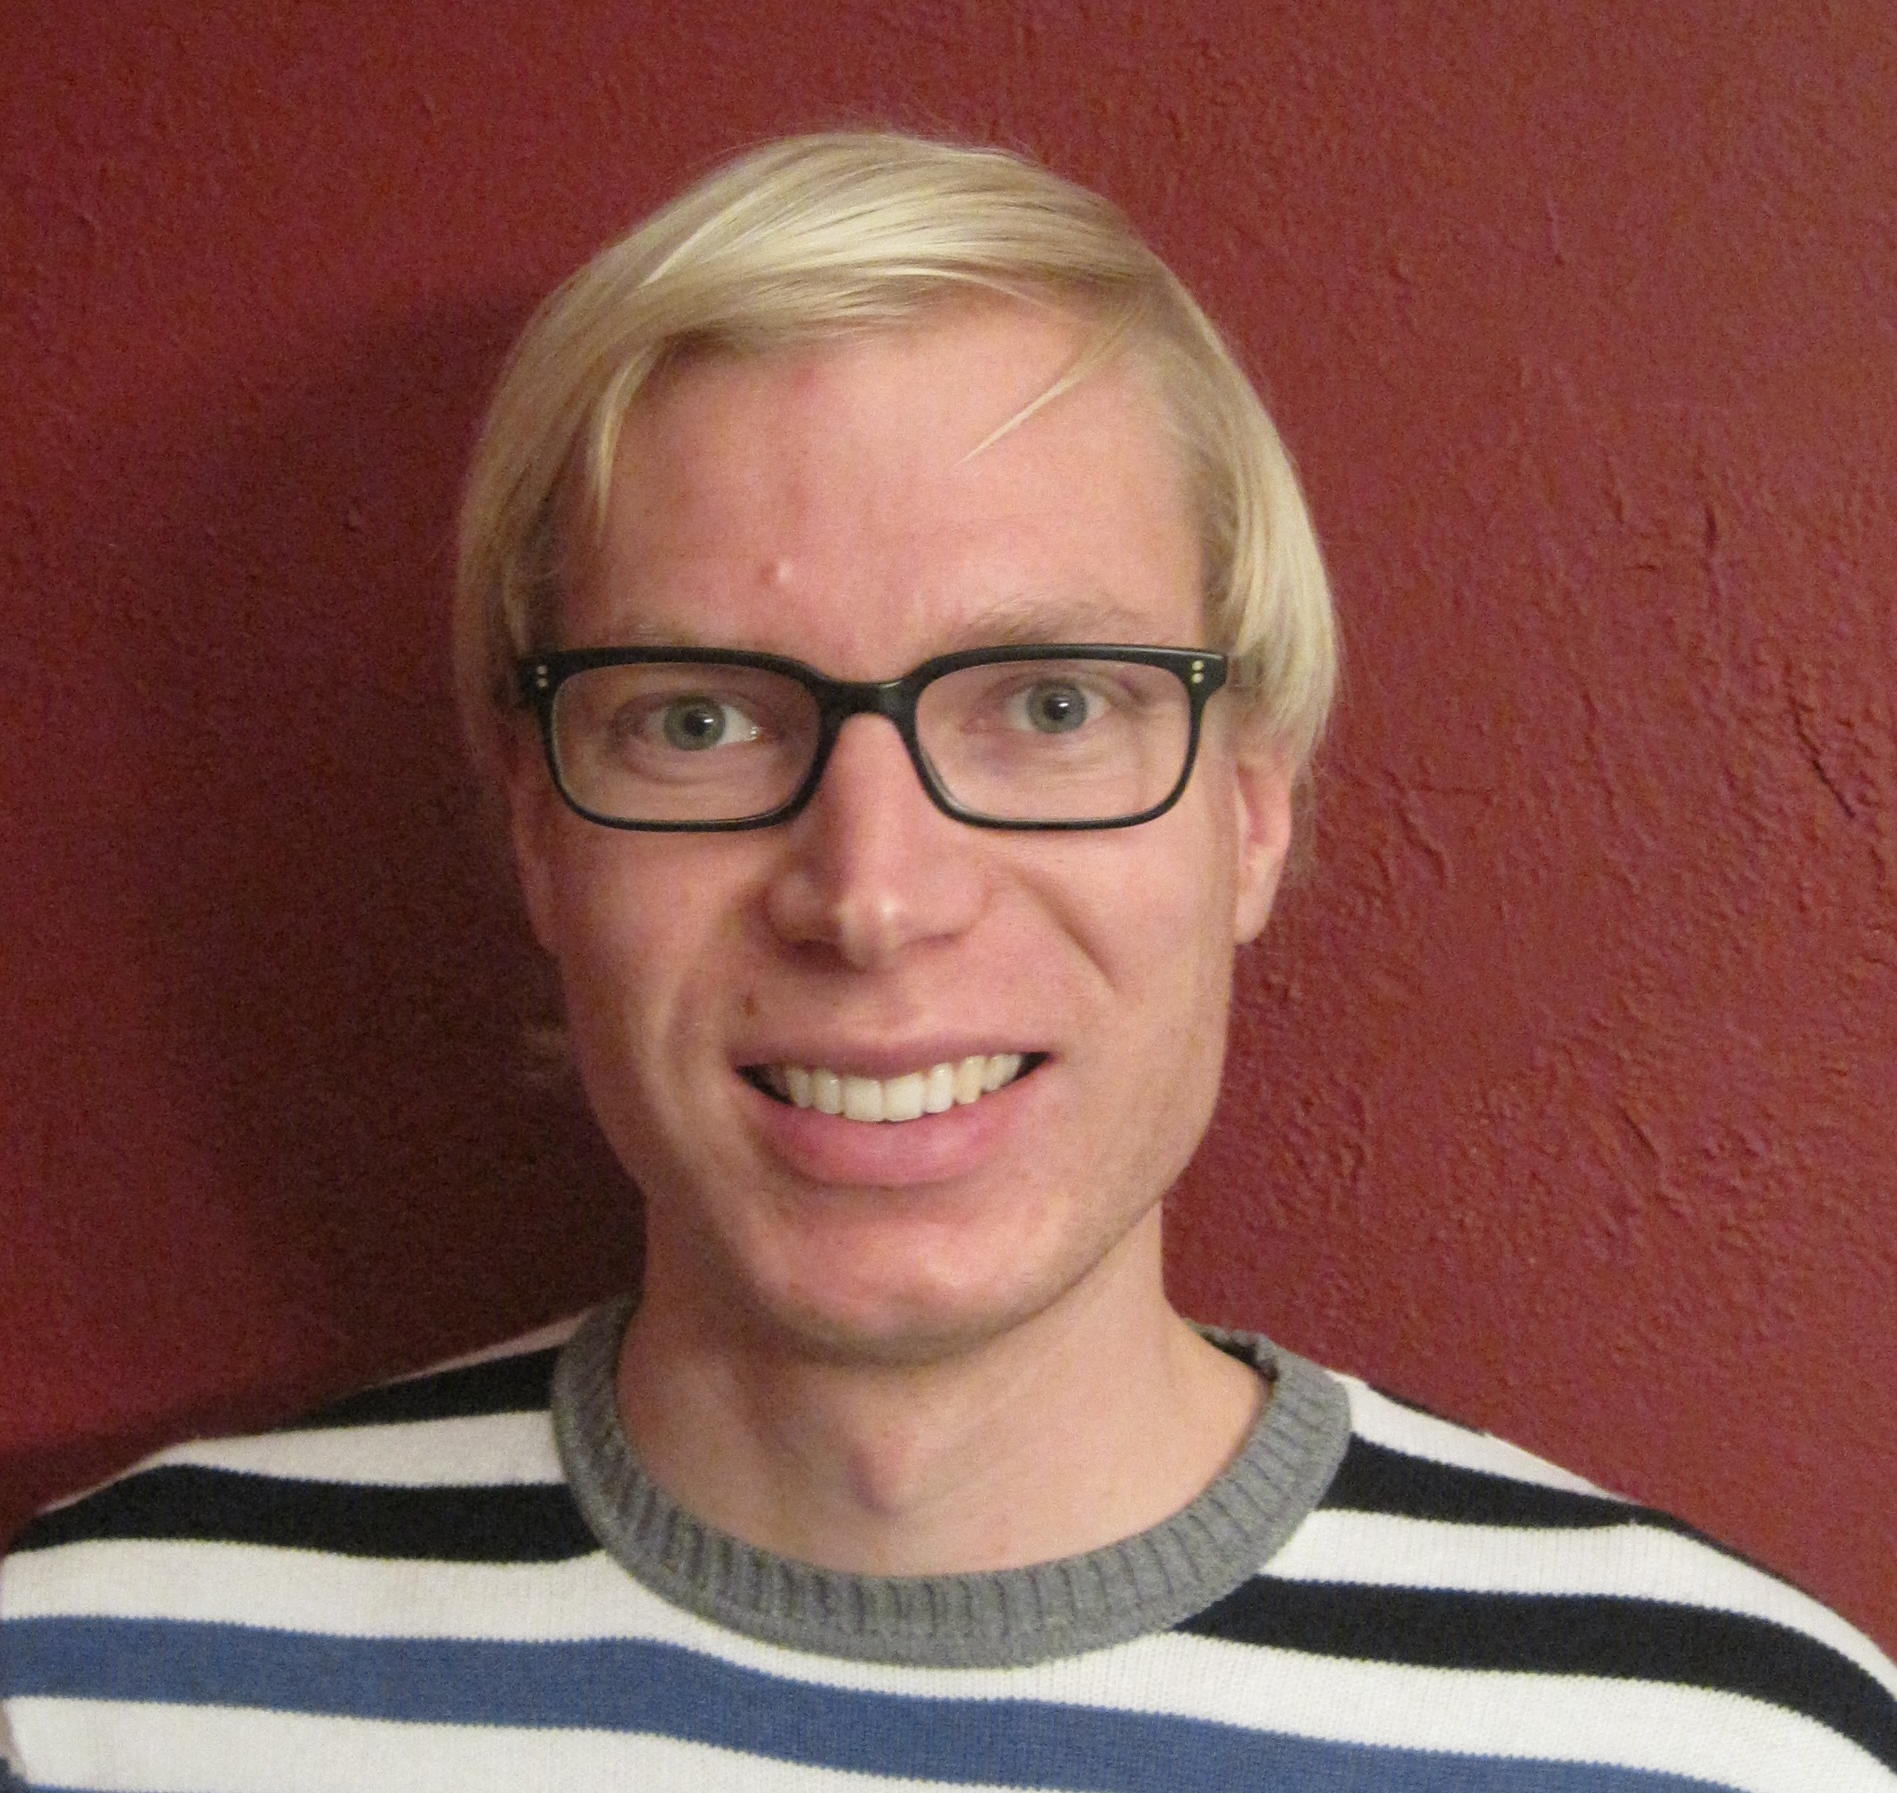
\includegraphics[width=1in,height=1.25in,clip,keepaspectratio]{figures/asend.png}}]{Nicholas
  Asendorf}
received the B.S. degree in computer engineering from the University of Maryland, College Park, MD, in 2010 and the M.S. degree in electrical engineering:systems from the University of Michigan in 2012.

He is a graduate student in the Department of Electrical Engineering and Computer Science at the University of Michigan, Ann Arbor. His research interests include the need for data driven algorithms in statistical signal processing and machine learning particularly in low SNR and sample starved settings.

\end{biography}

\begin{biography}[{\includegraphics[width=1in,height=1.25in,clip,keepaspectratio]{figures/nadak.jpg}}]{Raj Rao Nadakuditi}
is an Assistant Professor in the Department of Electrical Engineering and Computer Science at the University of Michigan. He received his PhD in 2007 from the Massachusetts Institute of Technology and the Woods Hole Oceanographic Institution. He was awarded an Office of Naval Research Young Investigator Award in 2011, an Air Force Office of Scientific Research Young Investigator Award in 2012 and the Signal Processing Society Best Young Author Paper Award in 2012. His research focuses on developing theory for random matrices for applications such in signal processing, machine learning, queuing theory and scattering theory. 
\end{biography}


% if you will not have a photo at all:
%\begin{IEEEbiographynophoto}{John Doe}
%Biography text here.
%\end{IEEEbiographynophoto}


% You can push biographies down or up by placing
% a \vfill before or after them. The appropriate
% use of \vfill depends on what kind of text is
% on the last page and whether or not the columns
% are being equalized.

%\vfill

% Can be used to pull up biographies so that the bottom of the last one
% is flush with the other column.
%\enlargethispage{-5in}




\end{document} 
